%Tipo de Documento [Conferencia]

\documentclass[conference]{IEEEtran}\usepackage[]{graphicx}\usepackage[]{color}
%% maxwidth is the original width if it is less than linewidth
%% otherwise use linewidth (to make sure the graphics do not exceed the margin)
\makeatletter
\def\maxwidth{ %
  \ifdim\Gin@nat@width>\linewidth
    \linewidth
  \else
    \Gin@nat@width
  \fi
}
\makeatother

\definecolor{fgcolor}{rgb}{0.345, 0.345, 0.345}
\newcommand{\hlnum}[1]{\textcolor[rgb]{0.686,0.059,0.569}{#1}}%
\newcommand{\hlstr}[1]{\textcolor[rgb]{0.192,0.494,0.8}{#1}}%
\newcommand{\hlcom}[1]{\textcolor[rgb]{0.678,0.584,0.686}{\textit{#1}}}%
\newcommand{\hlopt}[1]{\textcolor[rgb]{0,0,0}{#1}}%
\newcommand{\hlstd}[1]{\textcolor[rgb]{0.345,0.345,0.345}{#1}}%
\newcommand{\hlkwa}[1]{\textcolor[rgb]{0.161,0.373,0.58}{\textbf{#1}}}%
\newcommand{\hlkwb}[1]{\textcolor[rgb]{0.69,0.353,0.396}{#1}}%
\newcommand{\hlkwc}[1]{\textcolor[rgb]{0.333,0.667,0.333}{#1}}%
\newcommand{\hlkwd}[1]{\textcolor[rgb]{0.737,0.353,0.396}{\textbf{#1}}}%

\usepackage{framed}
\makeatletter
\newenvironment{kframe}{%
 \def\at@end@of@kframe{}%
 \ifinner\ifhmode%
  \def\at@end@of@kframe{\end{minipage}}%
  \begin{minipage}{\columnwidth}%
 \fi\fi%
 \def\FrameCommand##1{\hskip\@totalleftmargin \hskip-\fboxsep
 \colorbox{shadecolor}{##1}\hskip-\fboxsep
     % There is no \\@totalrightmargin, so:
     \hskip-\linewidth \hskip-\@totalleftmargin \hskip\columnwidth}%
 \MakeFramed {\advance\hsize-\width
   \@totalleftmargin\z@ \linewidth\hsize
   \@setminipage}}%
 {\par\unskip\endMakeFramed%
 \at@end@of@kframe}
\makeatother

\definecolor{shadecolor}{rgb}{.97, .97, .97}
\definecolor{messagecolor}{rgb}{0, 0, 0}
\definecolor{warningcolor}{rgb}{1, 0, 1}
\definecolor{errorcolor}{rgb}{1, 0, 0}
\newenvironment{knitrout}{}{} % an empty environment to be redefined in TeX

\usepackage{alltt}

%BIBLIOTECAS

% Este paquete se utiliza para generar texto o graficas de relleno.
%\usepackage{blindtext, graphicx}
%Biblioteca para graficas
\usepackage{graphicx}
%Biblioteca para lectura de caracteres ortográficos (tildes..etc. ) 
\usepackage[utf8]{inputenc}
%Biblioteca para enumeración de imagenes
\usepackage{float}
%Biblioteca para graficos vectrizados.svg 
\usepackage{svg}
\usepackage{enumerate}
%Biblioteca para enumerar figuras tablas.. etc en español 
\usepackage[spanish, es-tabla]{babel}
\usepackage[spanish]{babel}
%\usepackage[spanish,USenglish]{babel}

%INICIO DEL DOCUMENTO
\IfFileExists{upquote.sty}{\usepackage{upquote}}{}
\begin{document}
	
	
	% TITULO DEL PAPER
\title{Análisis de los Aportes al Sistema de Seguridad Social Colombiano con datos del DANE para el a\~no 2015}

% NOMBRE DE LOS AUTORES
\author{
	\IEEEauthorblockN{Fernando Buitrago }
		
	\IEEEauthorblockA{Universidad Distrital Francisco José de Caldas\\
		Bogotá D.C., Colombia\\
		Email: Fernadobuitragoa@gmail.com  }
	%\and
}
%TITULO
\maketitle

%abstract del documento
%Iniciar Abstract
\begin{abstract}
 This document contains a data analysis of the ``Online Retail'' dataset provided by the UCI Machine Learning Repository web site, this analysis is made to get knowledge from the transactions described in the dataset through a time line.
\end{abstract}

%Iniciar Palabras Clave Formato IEEE
\begin{IEEEkeywords}
	Linked Data, Data Mining, Dataset, Open Data.
\end{IEEEkeywords}

%Introduccion 
%SECCIÓN 1. INTRODUCCIÓN 
\section{Introducción}
	El gobierno de Colombia, ha liberado datos de ámbito general donde terceros puedan tener acceso a ellos, los utilicen y generen servicios de perfil social, fortaleciendo así la transparencia de la información gubernamental.
	Las aplicaciones de los resultados de los análisis de los datos abiertos tienen como propósito facilitar la toma de decisiones con mayor certidumbre de forma eficiente.
	En el presente artículo analizaremos datos publicados por el DANE basados en una encuesta realizada en el 2015 donde se representan los resultados a preguntas relacionadas con los aportes al sistema de seguridad social colombiano, los cuales serán abordados en este estudio. El alcance de esta revisión se limitará a dos variables: a) edad, b) Monto de los aportes al sistema de seguridad social Colombiano.
	\\

\section{Datos Abiertos}

Según el Ministerio de Tecnologías de la Información y las Comunicaciones de la República de Colombia MinTIC, los Datos Abiertos son todos aquellos datos primarios, sin procesar, en formatos estándar, estructurados e interoperables que facilitan su acceso y permiten su reutilización, los cuales están bajo la custodia de las entidades públicas y que pueden ser obtenidos y ofrecidos sin reserva alguna, de forma libre y sin restricciones, con el fin que terceros puedan reutilizarlos y crear servicios derivados de los mismos.
\\
Los datos abiertos se caracterizan por lo siguiente:
  \begin{itemize}
  	\item \textbf{Disponibilidad y acceso}: la información debe estar disponible como un todo y a un costo razonable de reproducción, preferiblemente descargándola de internet. Además, la información debe estar disponible en una forma conveniente y modificable.
  	
	\item \textbf{Reutilización y redistribución}: los datos deben ser provistos bajo términos que permitan reutilizarlos y redistribuirlos, e incluso integrarlos con otros conjuntos de datos.
	
	\item \textbf{Participación universal}: todos deben poder utilizar, reutilizar y redistribuir la información. No debe haber discriminación alguna en términos de esfuerzo, personas o grupos. Restricciones “no comerciales” que prevendrían el uso comercial de los datos; o restricciones de uso para ciertos propósitos (por ejemplo sólo para educación) no son permitidos. (Public.Resource.Org, 2007).
	
  \end{itemize}

Los datos abiertos se representan de tal manera que permitan a los diversos países alcanzar sus metas tanto estratégicas como operativas pretendiendo “generar servicios de valor agregado a la sociedad, a través del desarrollo de aplicaciones realizadas por terceros (comunidades de desarrollo, industria infomediaria y academia), que utilizan los datos abiertos generados por las entidades de los diversos Estados”. 

El modelo de datos abiertos definido por el estado colombiano, tiene como principales componentes “los objetivos asociados a la implementación de los mismos en el país,  los principios de diseño en las  diferentes  perspectivas, el  modelo específico  con  los elementos  estratégicos,  tácticos,  operativos  y  de  soporte  y por último, el  mapa  de  ruta que  define  las  acciones  puntuales  a ejecutar para apropiar el modelo de datos abiertos definido”.

Una de las entidades del estado Colombiano que está a la vanguardia en el tema de datos abiertos es el Departamento Administrativo de Estadística DANE, el cual a la fecha ha puesto a disposición de público su información en formato de microdatos o Datos Enlazados, también conocidos como Linked Data LD, los cuales presentan la propiedad de vincularse de manera distribuida en la Web, de tal forma que se pueden referenciar al igual que lo hacen los enlaces de las páginas web (W3C.es, 2012).

Si bien el objeto de este artículo son el análisis de los datos abiertos expuestos por el DANE, actualmente este tema ha evolucionado en Datos Abiertos Enlazados, también conocidos como Linked Open Data LOD, que consisten en la simbiosis de los Datos Abiertos (Open Data) y los Datos Enlazados (Linked Data). 

El consorcio que define los estándares para la web, conocido como W3C, ha publicado en su glosario que los datos abiertos enlazados son un conjunto de datos que se encuentran asociados y disponibles en la Web pública, al igual que cuentan con licenciamiento abierto para su reutilización. La publicación de los datos abiertos enlazados en la web permite realizar consultas distribuidas sobre los conjuntos de datos, (2015e).

A partir del concepto de Datos Abiertos, entre el 7 y 8 de diciembre de 2007 se reunieron 30 defensores de gobierno abierto para desarrollar un conjunto de principios de los Datos de Gobierno Abierto, los cuales son también conocidos como Open Government Data OGD. Dicha reunión, celebrada en Sebastopol, California, fue diseñada para desarrollar una comprensión más sólida de por qué los datos del gobierno abierto son esenciales para la democracia (Public.Resource.Org, 2007).

La publicación de datos abiertos gubernamentales en internet ha sido definida por el Consorcio de la W3C (2009), en tres pasos sencillos:

  \begin{itemize}
  
  	\item Paso 1: publicación de los datos en su forma cruda. Los datos deben estar bien estructurados, lo cual permite que otros hagan uso automatizado de los datos con éxito, en formatos o estructuras conocidas (v.g. XML, RDF y CSV) facilitando ver los datos, en lugar de extraerlos (por ejemplo, imágenes de los datos), lo que debe evitarse por no ser útil (ibid).

	\item Paso 2: Crear un catálogo en línea de los datos en bruto (completo y con documentación) para que las personas puedan descubrir lo que se ha publicado. Estos conjuntos de datos en bruto deben ser estructurados y documentados de forma fiable, de lo contrario su utilidad es insignificante.

	\item Paso 3: Los datos han de ser legibles tanto por los humanos como por las máquinas de la siguiente manera:

		\begin{itemize}
			\item Codificar los datos utilizando estándares abiertos y de la industria o crear sus propias normas en base a su vocabulario.
			\item Que sus datos legibles puedan convertirse por cualquier persona o mediante el uso de transformaciones por software en tiempo real siguiendo los requisitos de accesibilidad.
			\item Utilizar de manera permanente identificadores normalizados y detectables.
			\item Permitir citaciones electrónicas en forma de hipervínculos estandarizados
		\end{itemize}
	\end{itemize}	

Estos pasos le ayudarán al público a encontrar, usar, citar y comprender los datos fácilmente. El catálogo de datos debe explicar las reglas o reglamentos que deben seguirse en el uso del conjunto de datos. Además, el catálogo de datos en sí se consideran "datos y debe ser publicado como datos estructurados, por lo que terceras personas pueden extraerlos sobre los dichos conjuntos.



%Metodologia
%SECCIÓN 3. METODOLOGIA
\section{METODOLOGÍA}



 Para abordar el análisis de este problema se desarrollaran las siguientes tareas [1].
 
  \subsection{Reconocimiento de la información}
 
 El dataset utilizado en este análisis fue obtenido mediante una consulta sobre la base de datos de la Universidad de los Llanos y esta conformada por la información de los estudiantes activos de todas las facultades que componen la universidad.
  
  \begin{itemize}
   \item \textbf{Descripción la población}: La población objeto de este análisis esta compuesta por los estudiantes activos (matriculados) de la Universidad de los Llanos, que no poseen problemas académicos o administrativos; se excluyeron los estudiantes que pertenecen a primer semestre de todas las carreras de pregrado, debido a que no poseen promedio ponderado de carrera aún. 
   \bigskip
 
   La población esta compuesta por los datos de 5000 estudiantes que tiene la Universidad de los Llanos, los cuales fueron obtenidos mediante una consulta a la base de datos del sistema de registro y control académico de la Universidad de los Llanos, de donde se extrajeron en una hoja de calculo los siguientes campos:
   
   \item \textbf{Variables del DataSet:}\\
	    
	   \begin{itemize}
		   \item \textbf{ciudad}   : Ciudad de origen del estudiante
		   \item \textbf{dept} 	   : Departamento de origen del estudiante
		   \item \textbf{estrato}  : Estrato socieconomico del estudiante
		   \item \textbf{promedio} : Promedio ponderado de carrera del estudiante
		   \item \textbf{carrera}  : Programa académico que cursa el estudiante
		   \item \textbf{codigo}   : Código del estudiante
		   \item \textbf{nombre}   : Nombres y apellidos del estudiante
		   \item \textbf{genero}   : Genero del estudiante
		   \item \textbf{ingresos} : Ingresos del estudiante
		   \item \textbf{egresos}  : Egresos del estudiante
		   \item \textbf{identificacion}: Numero de identificación del estudiante
		\end{itemize}
	   
	   \item \textbf{Identificación del problema}: El estrato socio económico esta relacionado con la cantidad de dinero al que tiene acceso una persona para suplir sus necesidades materiales, pero existe algún tipo de relación entre el estrato socio económico y el desarrollo intelectual, particularmente aquel es medido a través del promedió ponderado de carrera en la Universidad de los Llanos\\ 
	    
	   \item \textbf{Objetivos}: Determinar si la situación socio económica (estrato socio económico) puede generar consecuencias directas sobre el rendimiento académico de los estudiantes de la Universidad de los Llanos.
   
  \end{itemize}
  \subsection{Preguntas de investigación}
  Las preguntas de investigación que se abordan en este análisis son las siguientes:
	  \begin{itemize}
	   \item ¿Existe algún tipo de relación entre el estrato socio económico y el desarrollo intelectual?
	   \item ¿Los estudiantes falsean el estrato social real, para obtener beneficios económicos en el valor de la matricula?
	   \item ¿La elección de estudiar en la Universidad de los Llanos, se realiza para reducir costos?
	   \item ¿La elección de estudiar en la Universidad de los Llanos, se realiza para obtener reconocimiento académico de la misma?
	  \end{itemize}
  \subsection{Análisis exploratorio}
    
  	Las variables que son objeto del análisis en esta investigación son el estrato socieconomico y el promedio ponderado de carrera, a continuación se realiza el análisis de cada una de ellas:
    	  
  \begin{itemize}
  	%alzate
	\item \textbf {Variable Estrato Socioeconomico}: Esta variable es un atributo de carácter ordinal, a la cual se le puede aplicar la frecuencia y la moda como medida de tendencia central y utilizar el diagrama de sectores o torta como forma de representación gráfica con el fin de establecer la distribución de cada estrato respecto al total de la población.  \\
	
	Los datos utilizados para analizar el comportamiento de la variable estrato socieconomico se resumen en la tabla de la Figura 1.
	
	\bigskip
	\begin{figure} [ht]
		\centering
		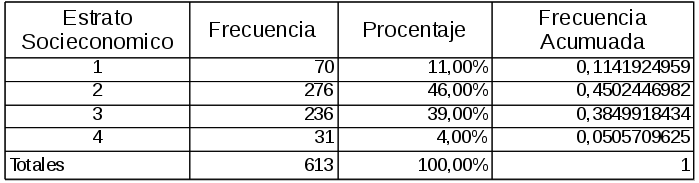
\includegraphics[width=0.9\linewidth]{figure/cuadro_socioeconomico}
		\caption{Variable Estrato Socioeconomico}
		\label{fig:cuadro_socioeconomico}
	\end{figure}

	En la Figura 2 se representa gráficamente la población por estrato utilizando diagramas de sectores o torta:  
	\bigskip

	\begin{figure} [ht]
		\centering
		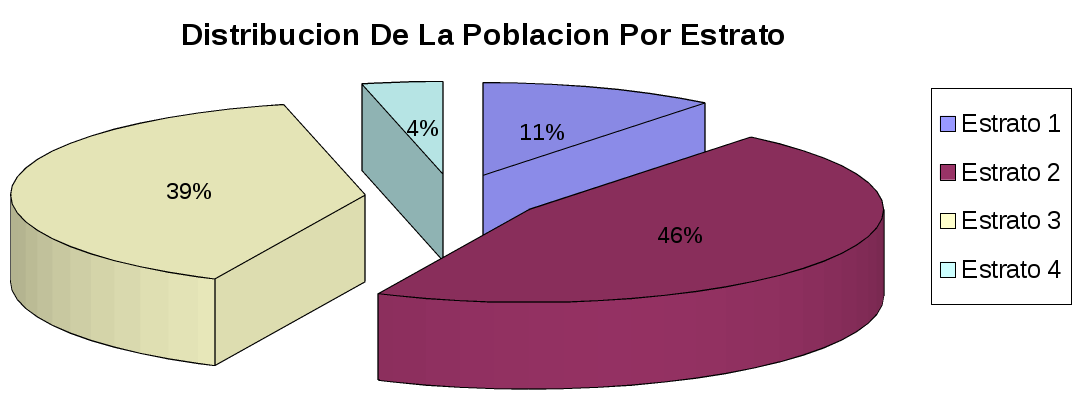
\includegraphics[width=0.9\linewidth]{figure/diagrama_sectores}
		\caption{Diagrama de sectores}
		\label{fig:diagrama_sectores}
	\end{figure}

	Como se puede observar en el diagrama de sectores la mayor cantidad de observaciones se encuentran agrupadas en el estrato 2 con un porcentaje de ocurrencia del 46\%.\\
	   
	Como se puede observar en el diagrama de barras de la Figura 3, la mayor cantidad de observaciones en la población ocurren en el estrato 2 con una frecuencia de 275 que corresponde al estrato hacia el que tienden a agruparsen las observaciones.
   
	\begin{figure}[ht]
		\centering
\begin{kframe}
\begin{alltt}
        \hlkwd{with}\hlstd{(datosep,} \hlkwd{hist}\hlstd{(estrato,} \hlkwc{breaks}\hlstd{=}\hlstr{"Sturges"}\hlstd{,} \hlkwc{col}\hlstd{=}\hlstr{"darkgray"}\hlstd{,} \hlkwc{main}\hlstd{=}\hlstr{"Diagrama de barras"}\hlstd{))}
\end{alltt}
\end{kframe}
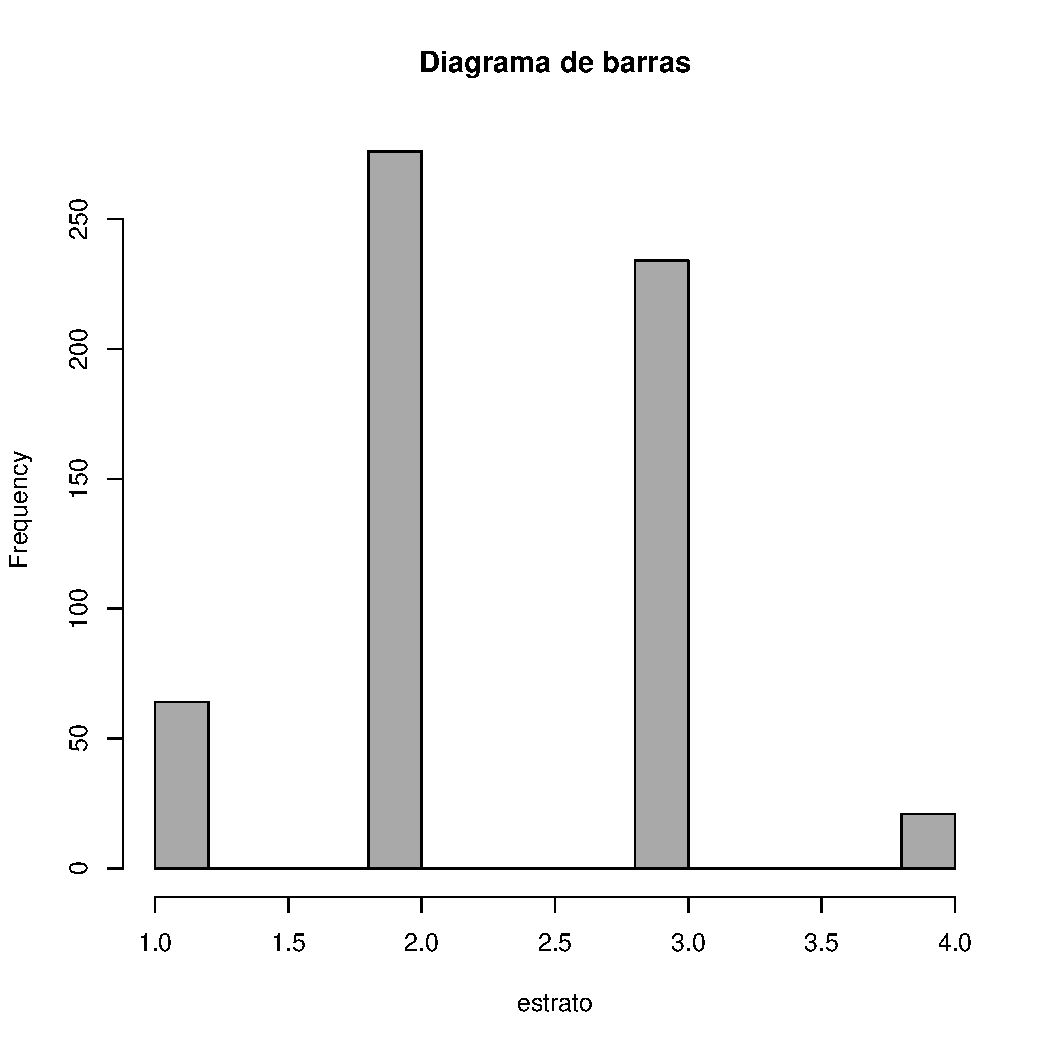
\includegraphics[width=\maxwidth]{figure/estrato-1} 

		\caption{Diagrama para estrato socioeconómico}
		\label{fig:diagrama_barras}
	\end{figure}

  	\item \textbf {Variable Promedio Ponderado de Carrera:}
	El promedio ponderado de carrera es una variable de carácter cuantitativo de tipo continuo, a la que se le puede aplicar la media y la mediana como medidas de tendencia central, a continuación se presentan los resultados.
	
\begin{kframe}
\begin{alltt}
        \hlstd{dfull} \hlkwb{<-} \hlkwd{data.frame}\hlstd{(}\hlkwc{Estrato}\hlstd{=datosep}\hlopt{$}\hlstd{estrato)}
        \hlkwd{stargazer}\hlstd{(dfull,} \hlkwc{type}\hlstd{=}\hlstr{"latex"}\hlstd{,} \hlkwc{title}\hlstd{=}\hlstr{"Promedio academico ponderado"}\hlstd{)}
\end{alltt}
\end{kframe}
% Table created by stargazer v.5.2 by Marek Hlavac, Harvard University. E-mail: hlavac at fas.harvard.edu
% Date and time: vie, jun 03, 2016 - 00:02:04
\begin{table}[!htbp] \centering 
  \caption{Promedio academico ponderado} 
  \label{} 
\begin{tabular}{@{\extracolsep{5pt}}lccccc} 
\\[-1.8ex]\hline 
\hline \\[-1.8ex] 
Statistic & \multicolumn{1}{c}{N} & \multicolumn{1}{c}{Mean} & \multicolumn{1}{c}{St. Dev.} & \multicolumn{1}{c}{Min} & \multicolumn{1}{c}{Max} \\ 
\hline \\[-1.8ex] 
Estrato & 595 & 2.356 & 0.718 & 1 & 4 \\ 
\hline \\[-1.8ex] 
\end{tabular} 
\end{table} 

	
	Se construyeron 5 intervalos de frecuencia de clase con el fin de facilitar el tratamiento y representación de los 613 promedios de carrera de los estudiantes de pregrado de la Universidad de los Llanos, los cuales se muestran a continuación:
	%\bigskip
	
	\begin{itemize}
		\item Intervalo 1: promedios de carrera entre 0 y 1  
		\item Intervalo 2: promedios de carrera entre 1,1 y 2
		\item Intervalo 3: promedios de carrera entre 2,1 y 3
		\item Intervalo 4: promedios de carrera entre 3,1 y 4 
		\item Intervalo 5: promedios de carrera entre 4,1 y 5
	\end{itemize}
%	\bigskip
		
	La tabla de frecuencias de la Figura 4 muestra el comportamiento de la variable promedio ponderado respecto a cada uno de los intervalos de clase.	
	
	\begin{figure}[ht]
		\centering
		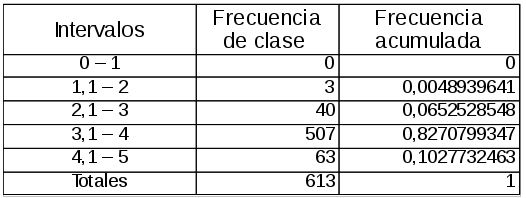
\includegraphics[width=0.7\linewidth]{figure/cuadro_promedio}
		\caption{Variable Promedio Ponderado de Carrera}
		\label{fig:cuadro_promedio}
	\end{figure}
	La Figura 5 representa gráficamente el comportamiento de la variable promedio ponderado de carrera mediante histograma de frecuencias de clases.

	\begin{figure}[ht]
		\centering
\begin{kframe}
\begin{alltt}
        \hlkwd{with}\hlstd{(datosep,} \hlkwd{hist}\hlstd{(promedio,} \hlkwc{breaks}\hlstd{=}\hlstr{"Sturges"}\hlstd{,} \hlkwc{col}\hlstd{=}\hlstr{"darkgray"}\hlstd{,} \hlkwc{main}\hlstd{=}\hlstr{"Histograma de frecuencias de clases"}\hlstd{))}
\end{alltt}
\end{kframe}
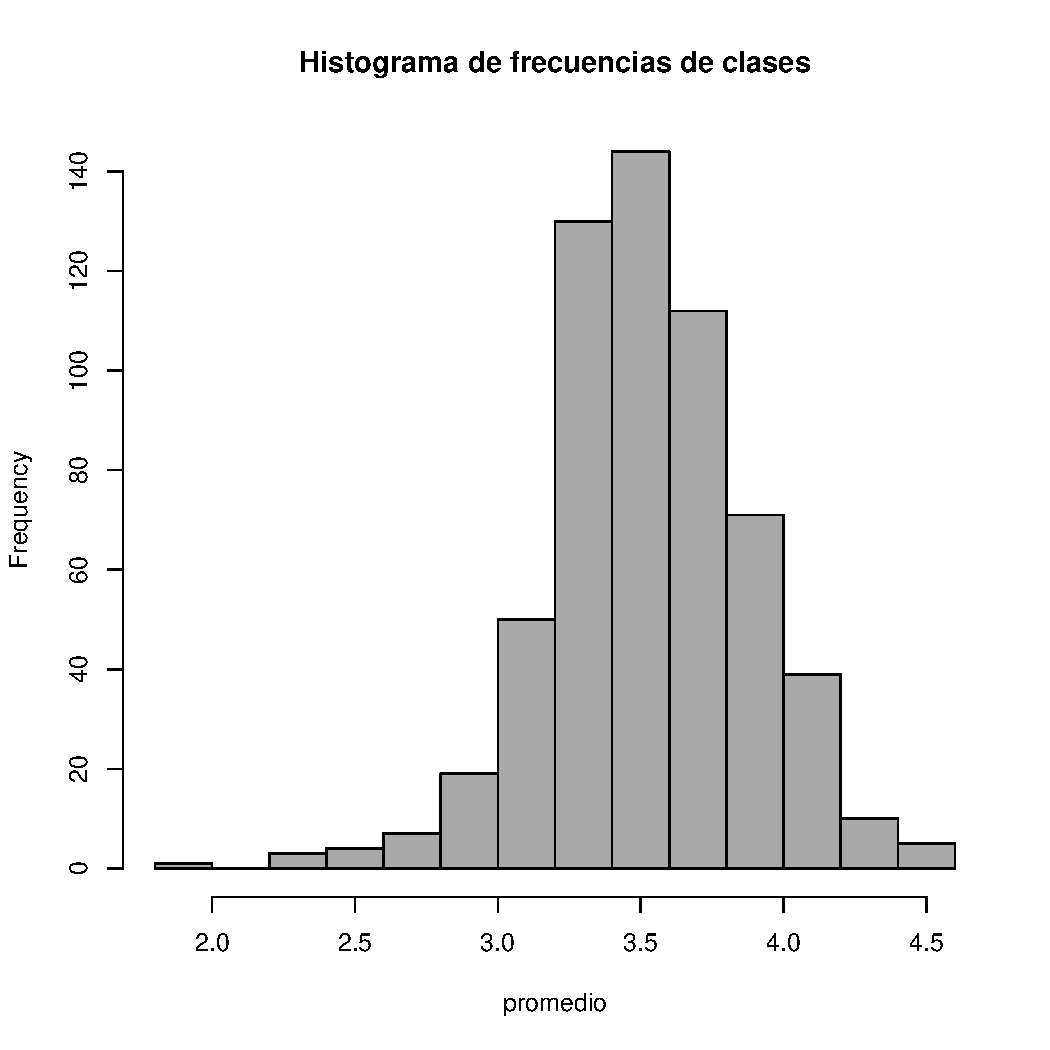
\includegraphics[width=\maxwidth]{figure/barrapromedio-1} 

		\caption{Histograma para Promedio Académico}
		\label{fig:barras_promedio_frecuencias_clase}
	\end{figure}

%	\begin{figure}[ht]
%		\centering
%		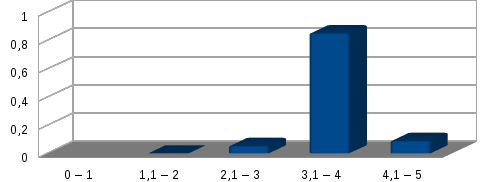
\includegraphics[width=0.9\linewidth]{figure/diagrama_barras_promedio}
%		\caption{Histograma Frecuencias Relativas}
%		\label{fig:diagrama_barras_promedio}
%	\end{figure}

	La Figura 6 muestra gráficamente la estimación de densidad para la variable promedio ponderado de carrera, lo que sugiere que los datos siguen una distribución normal y que se puede aplicar un estimador con base en la media o la varianza. 
	\begin{figure}[ht]
		\centering
\begin{kframe}
\begin{alltt}
        \hlkwd{densityplot}\hlstd{(} \hlopt{~} \hlstd{promedio,} \hlkwc{data}\hlstd{=datosep,} \hlkwc{bw}\hlstd{=}\hlstr{"SJ"}\hlstd{,} \hlkwc{adjust}\hlstd{=}\hlnum{1}\hlstd{,} \hlkwc{kernel}\hlstd{=}\hlstr{"epanechnikov"}\hlstd{,}  \hlkwc{main}\hlstd{=}\hlstr{"Diagrama de estimación de densidad"}\hlstd{)}
\end{alltt}
\end{kframe}
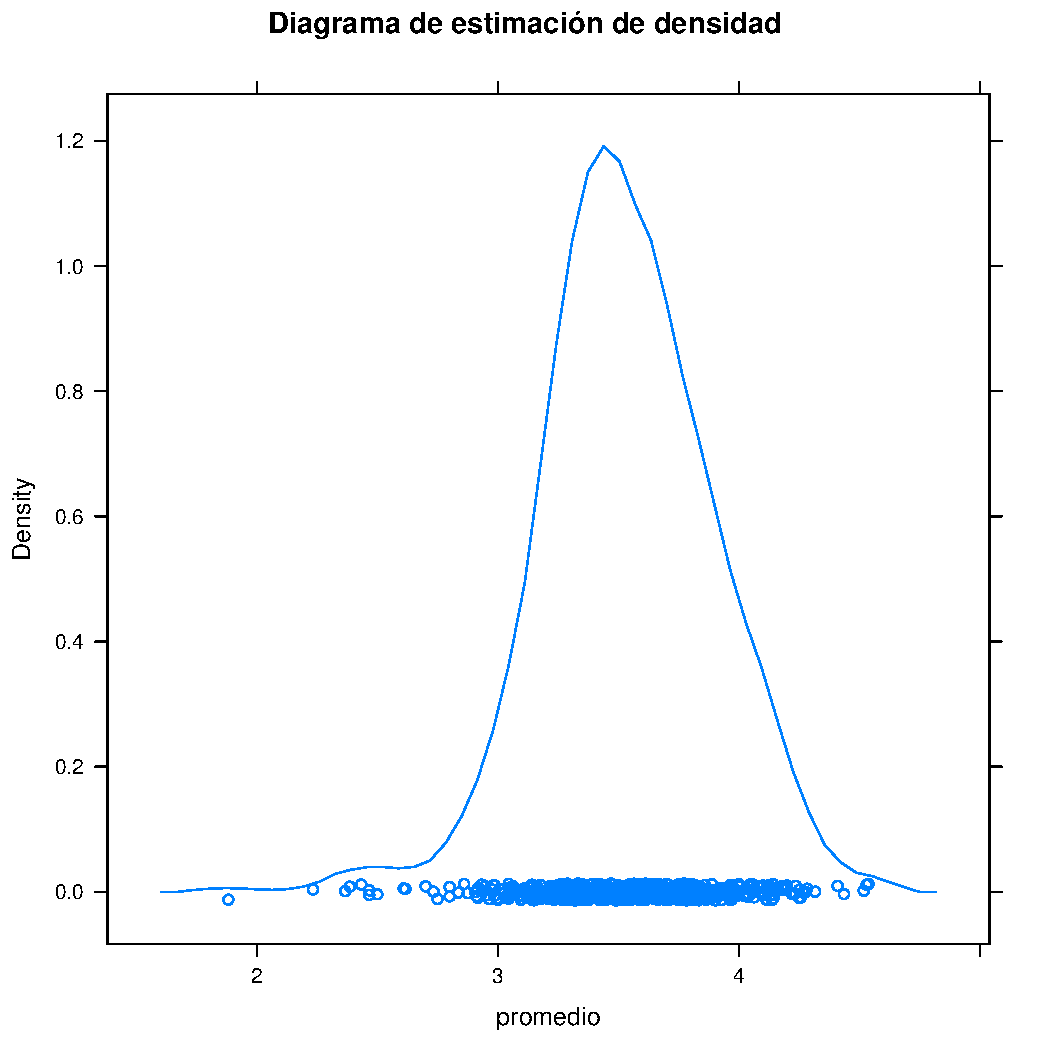
\includegraphics[width=\maxwidth]{figure/densidad-1} 
\begin{kframe}\begin{alltt}
        \hlcom{#densityplot( ~ promedio, data=datosep, bw="SJ", adjust=1, kernel="biweight")}
        \hlcom{#densityplot( ~ promedio, data=datosep, bw="SJ", adjust=1, kernel="gaussian")}
\end{alltt}
\end{kframe}
		\caption{Estimación de densidad para Promedio Académico}
		\label{fig:estimacion_frecuencia:promedio}
	\end{figure}

	\begin{figure}[ht]
		\centering
\begin{kframe}
\begin{alltt}
        \hlkwd{stripchart}\hlstd{(datosep}\hlopt{$}\hlstd{promedio,} \hlkwc{method}\hlstd{=}\hlstr{"stack"}\hlstd{,} \hlkwc{xlab}\hlstd{=}\hlstr{"Promedio ponderado Academico"}\hlstd{,} \hlkwc{main}\hlstd{=}\hlstr{"Diagrama de caja"}\hlstd{)}
\end{alltt}
\end{kframe}
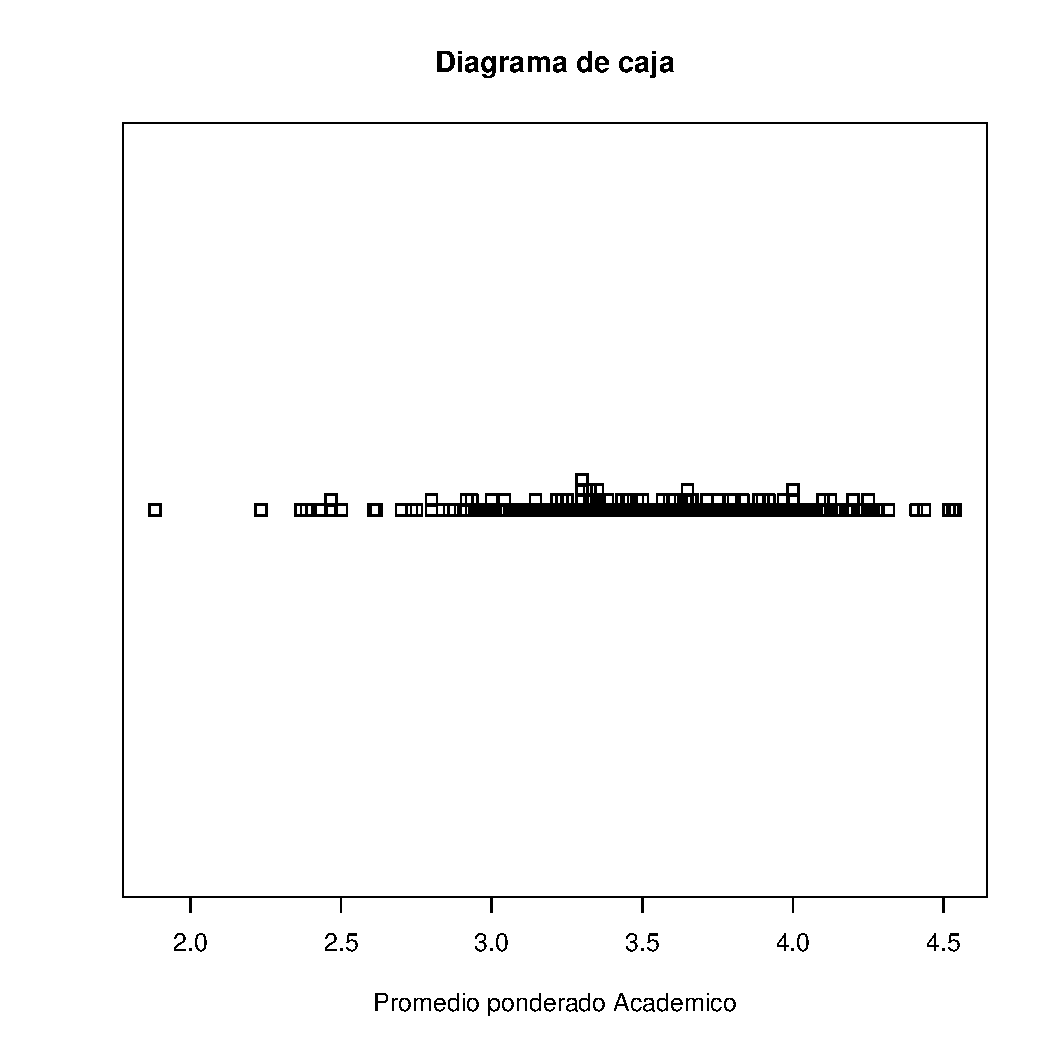
\includegraphics[width=\maxwidth]{figure/diagrama_puntos-1} 

		\caption{Diagrama de puntos para Promedio Académico}
		\label{fig:diagrama_puntos}
	\end{figure}

	Al aplicar la prueba de Shapiro-Wilk para validar el comportamiento de normal de los datos, se obtiene una confianza de W=0,9857 y p-value 0,0001457, como el valor de confianza deseado es 0,05 y el valor obtenido es menor se afirma que los datos no se comportan de forma normal.
	
	\begin{center}
		\bigskip
\begin{kframe}
\begin{alltt}
        \hlkwd{with}\hlstd{(datosep,} \hlkwd{shapiro.test}\hlstd{(promedio))}
\end{alltt}
\end{kframe}
	Shapiro-Wilk normality test

data:  promedio
W = 0.9857, p-value = 1.457e-05


	\end{center}
			
	\bigskip
	La Figura 7 muestra el diagrama de caja (box plot) que se construyo para visualizar gráficamente los datos atípicos que impiden que los datos alcancen el comportamiento normal.
		
	\begin{figure}[ht]
		\centering
\begin{kframe}
\begin{alltt}
        \hlkwd{boxplot}\hlstd{(datosep}\hlopt{$}\hlstd{promedio,} \hlkwc{data}\hlstd{=datosep,} \hlkwc{xlab}\hlstd{=}\hlstr{"Promedio Ponderado Academico"}\hlstd{,} \hlkwc{ylab}\hlstd{=}\hlstr{"Rango de calificación"}\hlstd{,} \hlkwc{id.method}\hlstd{=}\hlstr{"y"}\hlstd{,} \hlkwc{main}\hlstd{=}\hlstr{"Diagrama de caja"}\hlstd{)}
\end{alltt}
\end{kframe}
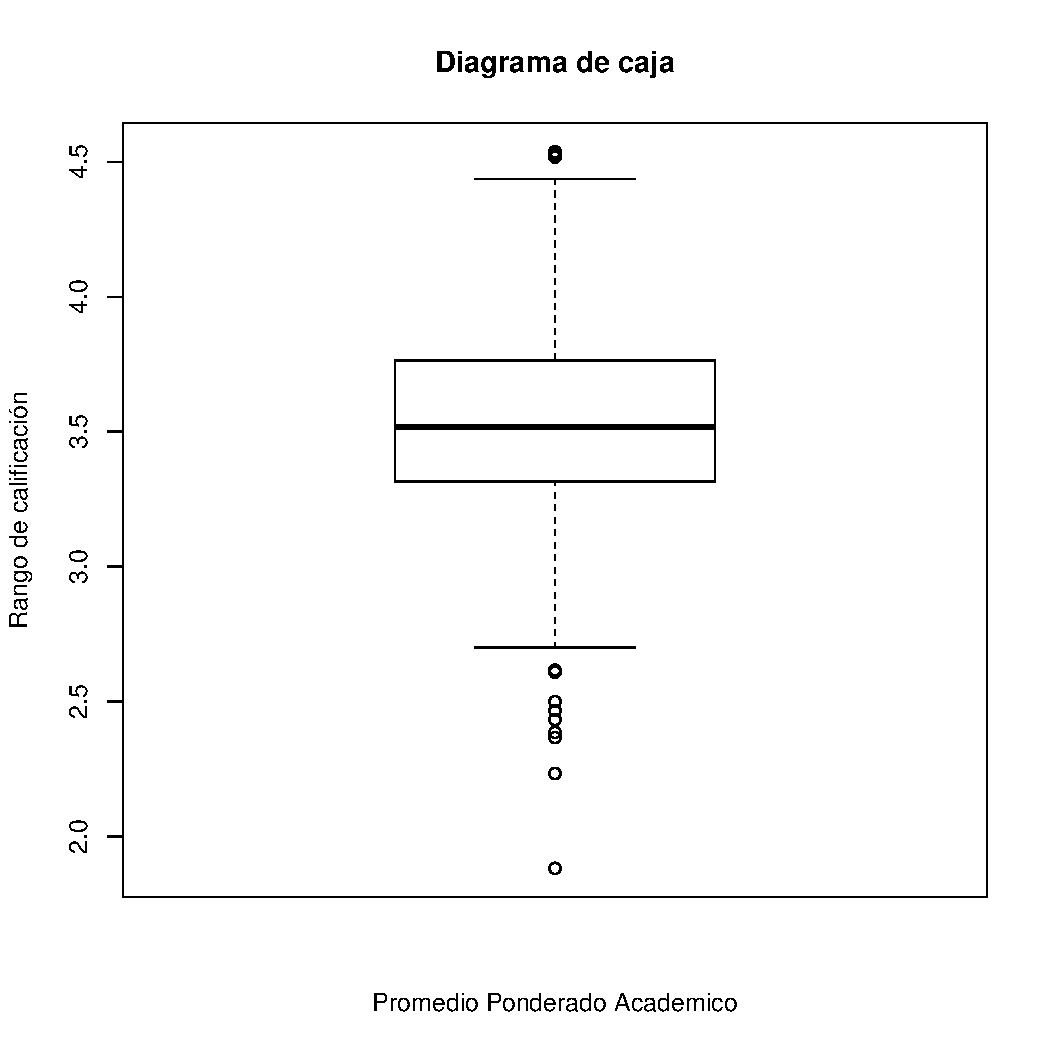
\includegraphics[width=\maxwidth]{figure/boxplot-1} 

		\caption{Diagrama de caja de la variable promedio}
		\label{fig:diagrama_boxplot_promedio}
	\end{figure}
	
	\bigskip

	Se aplica la técnica de truncamiento para forzar que los datos se comporten de forma normal, para ello se ordenan los datos de mayor a menor y se eliminan 150 datos, 75 en cada extremo. \\
	
	Se aplica nuevamente la prueba de normalidad de Shapiro-Wilk, obteniendo esta vez un comportamiento de normalidad en los datos resultados:\\
	
	\begin{center}
\begin{kframe}
\begin{alltt}
        \hlkwd{with}\hlstd{(datosept,} \hlkwd{shapiro.test}\hlstd{(promedio))}
\end{alltt}
\end{kframe}
	Shapiro-Wilk normality test

data:  promedio
W = 0.9857, p-value = 3.387e-05


	\end{center}
	\bigskip	
	Se realiza nuevamente el diagrama de caja (box plot) y se confirma que ya no existen datos outline o atípicos.
	
	\begin{figure}[ht]
		\centering
\begin{kframe}
\begin{alltt}
        \hlkwd{boxplot}\hlstd{(datosept}\hlopt{$}\hlstd{promedio,} \hlkwc{data}\hlstd{=datosept,} \hlkwc{xlab}\hlstd{=}\hlstr{"Promedio Ponderado Academico"}\hlstd{,} \hlkwc{ylab}\hlstd{=}\hlstr{"Rango de calificación"}\hlstd{,} \hlkwc{id.method}\hlstd{=}\hlstr{"y"}\hlstd{,} \hlkwc{main}\hlstd{=}\hlstr{"Diagrama de caja"}\hlstd{)}
\end{alltt}
\end{kframe}
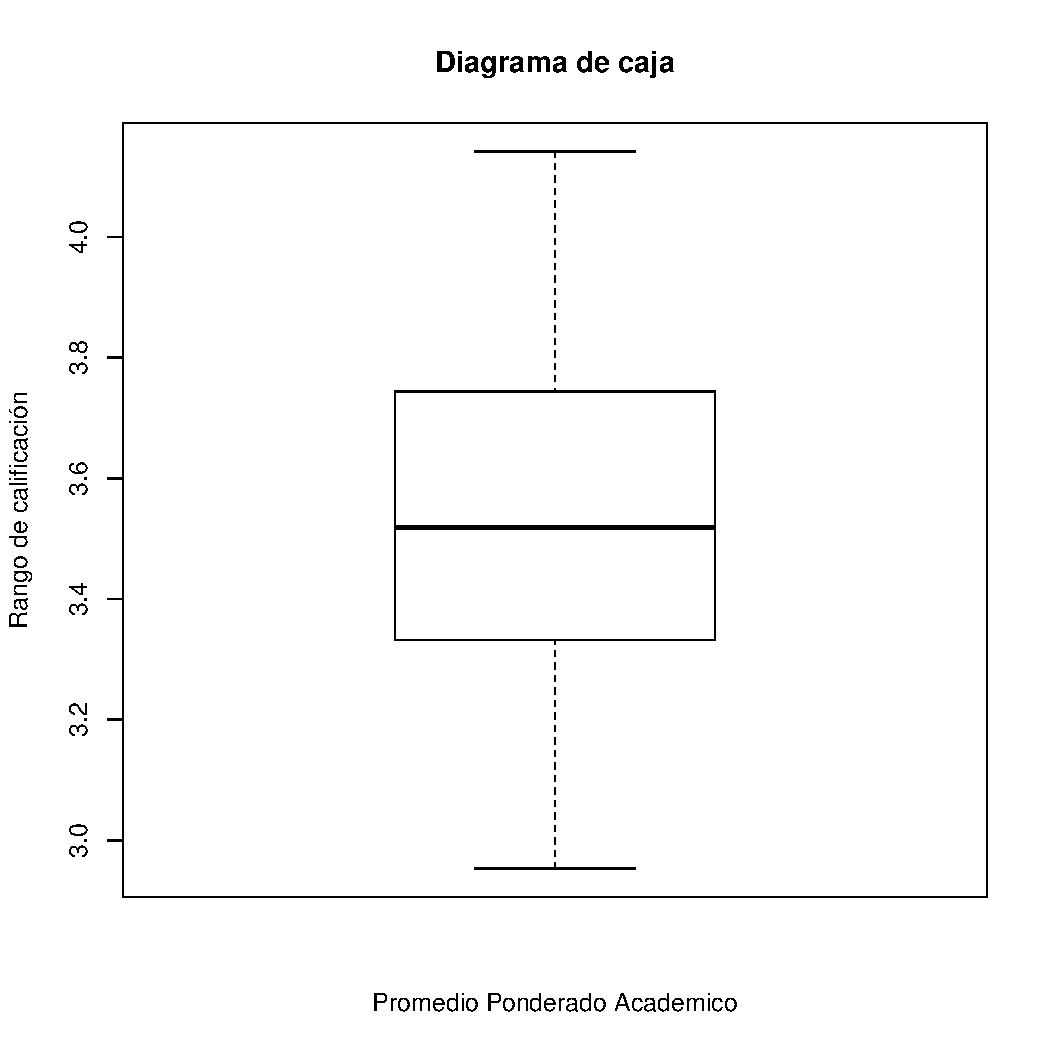
\includegraphics[width=\maxwidth]{figure/boxplot_trucado-1} 

		\caption{Diagrama de caja de la variable promedio truncada}
		\label{fig:diagrama_boxplot_promedio_truncada}
	\end{figure}
		
	\begin{figure}[ht]
		\centering
\begin{kframe}
\begin{alltt}
        \hlcom{#xyplot(promedio ~ estrato, type="p", pch=16, auto.key=list(border=TRUE), par.settings=simpleTheme(pch=16), scales=list(x=list(relation='same'), y=list(relation='same')), data=datosep)}

        \hlcom{#scatterplot(datosep$promedio~datosep$estrato, reg.line=lm, smooth=TRUE, spread=TRUE, id.method='mahal', id.n = 2, boxplots='xy', span=0.5, data=datosep, main="Estimación de densidad")}

        \hlcom{#scatterplot(promedio~estrato, reg.line=lm, smooth=TRUE, spread=TRUE, id.method='mahal', id.n = 2, boxplots='xy', span=0.5, data=datosep, main="Estimación de densidad")}

        \hlkwd{ggplot}\hlstd{(datosep,}\hlkwd{aes}\hlstd{(TPH),}\hlkwd{label}\hlstd{(}\hlstr{""}\hlstd{))} \hlopt{+} \hlkwd{geom_dotplot}\hlstd{()}
\end{alltt}


{\ttfamily\noindent\bfseries\color{errorcolor}{\#\# Error in eval(expr, envir, enclos): objeto 'TPH' no encontrado}}\end{kframe}
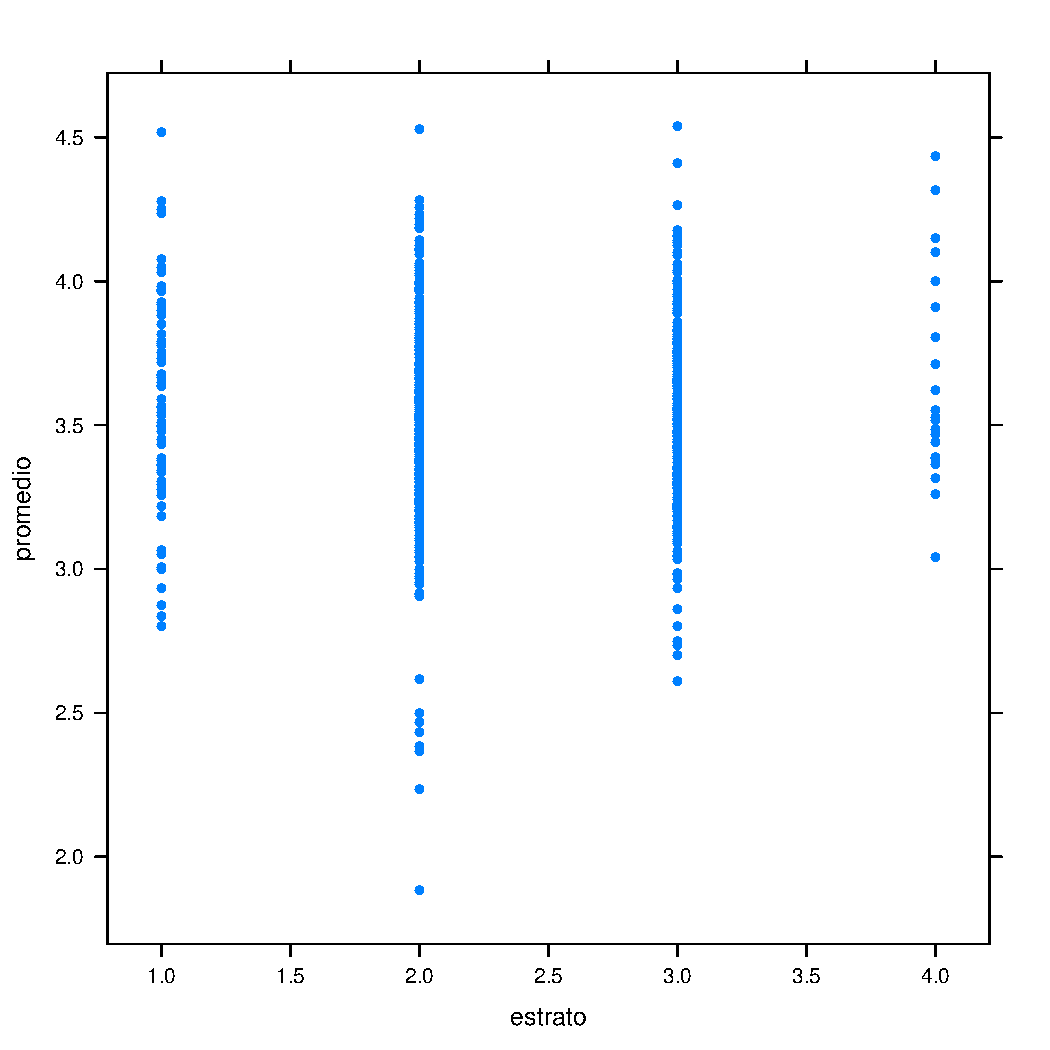
\includegraphics[width=\maxwidth]{figure/dispersion-1} 

		\caption{Diagrama de dispersión}
		\label{fig:diagrama_dispersion}
	\end{figure}
	
	\item \textbf {Diseño del espacio muestral:}
	El muestreo aplicado para abordar el análisis del dataset es Muestreo Aleatorio Simple (MAS) y el método utilizado para realizar la selección de los datos que conforman la muestra es coordinado negativo, a continuación se relacionan los cálculos realizados para obtener el tamaño de la muestra:
	\bigskip
	\begin{itemize}
		\item Asignar un numero aleatorio a cada dato de la muestra
		\item Ordenar de menor a mayor, de acuerdo al dato aleatorio cada elemento de la muestra
		\item Seleccionar desde primer dato hasta el tamaño de la muestra
	\end{itemize}
	\bigskip
	Los datos introducidos en los parámetros que proporciona la plantilla (documento adjunto) para calcular el tamaño de la muestra utilizando Muestreo Aleatorio Simple MAS, son los que se muestran a continuación:\\
	
	\begin{itemize}
		\item Tamaño de la población 	N = 5000	
		\item Error que se comete		E = 0,03	\\se recomienda que este entre 0,02 y 0,03
		\item Proporción del dominio	P = 0,30	\\P tomar valores entre 0 y 1
		\item Nivel de confianza		C = 0,91	\\(1 – alfa) donde alfa toma valores entre (0 y 1)
	\end{itemize}
	\bigskip
  	  	El tamaño de la muestra después de aplicar la técnica del coordinador negativo (M) es:
  	\bigskip  	
  	\begin{itemize}
  		\item Variabilidad			V = 0,2100420084
	  	\item Valor del percentil 	Z(alfa) = -1,6953977103
		\item Tamaño de la muestra 	M = 591  	
  	\end{itemize}
  	\bigskip  	
  	Una vez obtenido el tamaño de la muestra, se aplico la técnica de coordinador negativo a los datos de los estudiantes; el procedimiento realizado es el que se describe a continuación:
  	\bigskip
  	\begin{itemize}
  		\item Asigna un numero aleatorio a cada dato de la muestra
		\item Se ordena de menor a mayor con respecto a la asignación aleatoria 
		\item Se selecciona del primero hasta el tamaño de la muestra  
  	 \end{itemize}
  	\bigskip  		
  	Para el caso de los estudiantes de la Universidad de los Llanos se poseen los datos completos de toda la población objeto de análisis, pero con fin de corroborar la valides de los datos proporcionados mediante una encuesta, se calcula el tamaño de la muestra y se realiza la estimación bajo criterios de normalidad se selecciono una muestra de tamaño 613.
  	  	
   
  % \item Medidas de tendencia central[4] 
		 %15\
		 %\item Varianza [4] : La Varianza de las observaciones %$x_{1},x_{2},...,x_{n}$ es en esencia, el promedio del cuadrado %de las distancias entre cada observaci\'on y la media del %conjunto de observaciones. Se denota por:
		 %$$s^{2}=\sum_{i=1}^{n} \frac{ \left( %x_{i}-\overline{x}\right)^{2}}{\left(n-1 \right) } $$ 
		 
		 %\item Desviación estándar [4]: La desviaci\'on est\'andar es la %raiz cuadrada de la varianza y se denota por:
		 %$$s=\sqrt{\sum_{i=1}^{n} \frac{ \left( %x_{i}-\overline{x}\right)^{2}}{\left(n-1 \right) } }$$ 
		 		 
		 %Se puede aplicar una medida de tendencia central como la media y %un medida de dispersión  como la varianza. A continuación se %muestran los valores calculados para la variable promedio de %carrera ponderado.
%		 \begin{figure}[ht]
%			\centering
%			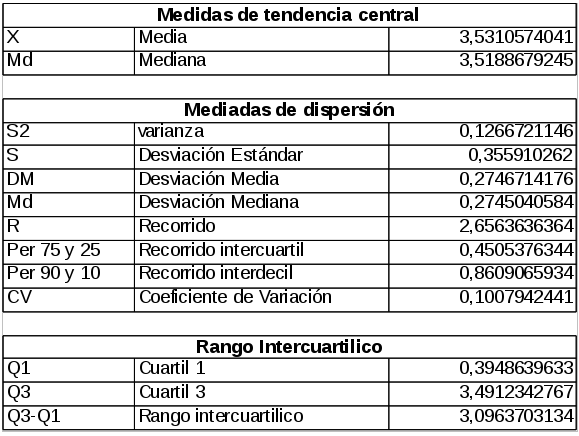
\includegraphics[width=0.9\linewidth]{figure/medidas_rpbabilidad}
%			\caption{}
%			\label{fig:medidas_rpbabilidad}
%		\end{figure}
 
\end{itemize} 


%Preguntas de investigacion
%SECCIÓN 3. PREGUNTAS INVESTIGACION


\section{Preguntas de investigación}
Las preguntas de investigación permitirán analizar el comportamiento de los datos basados en el dataset, ya que a través de ellas se logra una mejor interpretación  y definición del problema.  Las preguntas de investigación se clasifican en varios tipos de acuerdo al análisis que se desea lograr y en este caso se van a desarrollar las siguientes: Nota: Utilizando K-means se  categorizaron las datos. Ver pág. 8.
 \subsection{Preguntas de carácter descriptivo}
 Las preguntas de carácter descriptivo permiten identificar y conocer las características iniciales del conjunto de datos. Las preguntas de carácter descriptivo son:
  \begin{itemize}
  \item ¿Cuál es la Media de los montos de los aportes de los ciudadanos cuya edad está entre los 22 a los 26 años, 27 a los 50 años, 51 a los 71 años, y 72 a los 94 años?
  \item ¿Cuál es el mayor y menor monto aportando al Sistema de Seguridad Social con edad superior a 72 años?
  \item ¿Cuál es el mayor y menor monto aportando al Sistema de Seguridad Social con edad superior a 51 años?
  \item ¿Cuál es el mayor y menor monto aportando al Sistema de Seguridad Social con edad superior a 27 años?
  \item ¿Cuál es el mayor y menor monto aportando al Sistema de Seguridad Social con edad superior a 22 años? 

  \end{itemize}
  \subsection{Preguntas de caracter exploratorio}
   Las preguntas de carácter exploratorio consisten en la búsqueda de patrones o relaciones que soporten una pregunta de investigación.
  \begin{itemize}
   \item ¿El valor máximo de los aportes realizados por la población colombiana al sistema de seguridad social aumentan con relación a la variable Edad?


  \end{itemize}
  \subsection{Preguntas de caracter inferencial}
   Las preguntas de carácter inferencial consisten en el planteamiento de una hipótesis que podría ser resuelta con el análisis respectivo de la información
  \begin{itemize}
   \item ¿Los colombianos que más aportan al sistema son ciudadanos que tienen una edad mayor a 30 años?
  \end{itemize}



	
	% Analisis Datos DANE

\section{An\'{a}lisis de la Información del DANE}

A continuaci\'{o}n se presenta el an\'{a}lisis  de la informaciòn del DANE clasificada por la variable Edad del aportante.  Los datos han sido divididos en cinco grupos para determinar el comportamiento de los datos a trav\'{e}s del an\'{a}lisis de gr\'{a}ficos y de estad\'{i}stica b\'{a}sica para permitir explorar la distribuci\'{o}n de los datos e identificar caracter\'{i}sticas que resuleva la pregunta planteada durante la formulaci\'{o}n del problema.   

%Configuración de Clusters de Datos del DANE




\subsection{An\'{a}lisis inicial}
Lo primero que se analizar\'{a} es el comportamiento de los datos en las variables Total Aportantes, G\'{e}nero de los Aportantes y Edad del Aportante; obteniendo los siguientes resultados:
%\vspace{1mm}



% Table created by stargazer v.5.2 by Marek Hlavac, Harvard University. E-mail: hlavac at fas.harvard.edu
% Date and time: vie, jun 03, 2016 - 05:04:03 p.m.
\begin{table}[!htbp] \centering 
  \caption{Total Poblacion Analizada} 
  \label{} 
\begin{tabular}{@{\extracolsep{5pt}}lccccc} 
\\[-1.8ex]\hline 
\hline \\[-1.8ex] 
Statistic & \multicolumn{1}{c}{N} & \multicolumn{1}{c}{Mean} & \multicolumn{1}{c}{St. Dev.} & \multicolumn{1}{c}{Min} & \multicolumn{1}{c}{Max} \\ 
\hline \\[-1.8ex] 
TotalAportes & 42 & 140,206.500 & 170,046.000 & 98 & 890,000 \\ 
Genero & 99 & 1.535 & 0.501 & 1 & 2 \\ 
Edad & 99 & 40.253 & 22.909 & 2 & 94 \\ 
\hline \\[-1.8ex] 
\end{tabular} 
\end{table} 


%\vspace{1mm}
{\footnotesize \textbf{Convenciones:} Genero) 1: Mujer, 2: Hombre; Edad) Edad del Aportante Analizado.}

%\vspace{1mm}
El an\'{a}lisis principal de esta investigaci\'{o}n se enfoca en comprobar s\'{i} el monto de los aportes aumenta con relaci\'{o}n a la variable edad del aportante. En la revisi\'{o}n de los datos se evidencia que el valor de la media  est\'{a} m\'{a}s cerca del valor m\'{i}nimo  aportado al sistema de seguridad social colombiano.  Por tal raz\'{o}n se ha hace necesario ampliar el an\'{a}lisis a trav\'{e}s de un gr\'{a}fico para poder visualizar mejor los datos de la variable Edad del Aportante.   

\begin{figure}[H]
	\centering
\begin{knitrout}
\definecolor{shadecolor}{rgb}{0.969, 0.969, 0.969}\color{fgcolor}
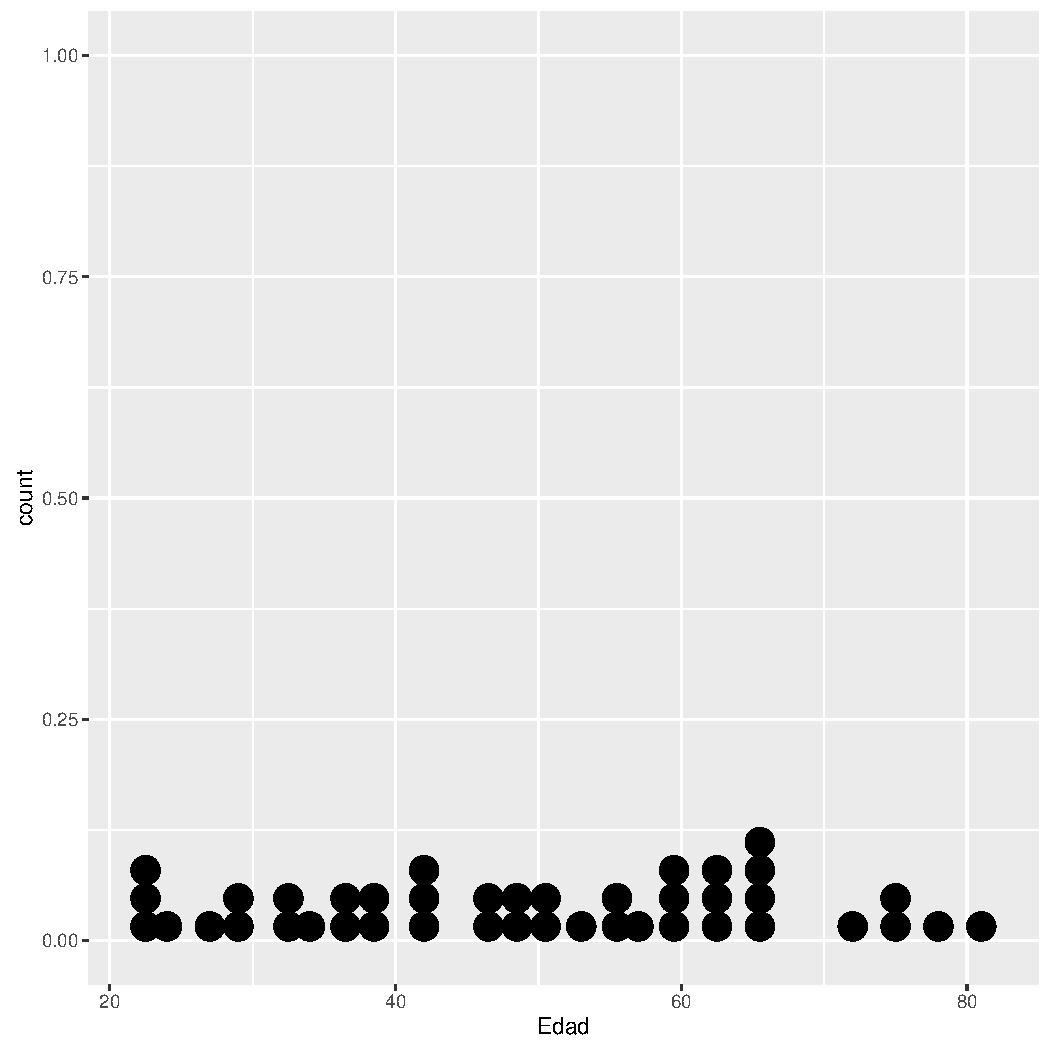
\includegraphics[width=\maxwidth]{figure/EdadAportante-1} 

\end{knitrout}
	\caption{Comportamiento de la variable Edad del Aportante}
\end{figure}

De acuerdo con los datos de la gr\'{a}fica, inicialmente se observan aportes a partir de 22 años, los cuales disminuyen hasta alcanzar 35 años. Posteriormente, el n\'{u}mero de aportante al sistema de seguridad social se mantiene entre el rango de 35 a 45 años.  Luego, la gr\'{a}fica presenta un aumento en el n\'{u}mero de aportantes hasta alcanzar la edad de 60 años. Finalmente, el n\'{u}mero de aportes disminuye hacia los 94 años. En consecuencia, basados en los resultados de los datos, el sistema de seguridad social colombiano est\'{a} financiado por aportes provenientes de ciudadanos que tienen una edad entre 22 hasta 94 años.

Tambi\'{e}n, analizaremos en la siguiente gr\'{a}fica, la distribuci\'{o}n de los datos relacionados con la variable montos de los aportes al sistema de seguridad social, observando lo siguiente:

\begin{figure}[H]
	\centering
\begin{knitrout}
\definecolor{shadecolor}{rgb}{0.969, 0.969, 0.969}\color{fgcolor}
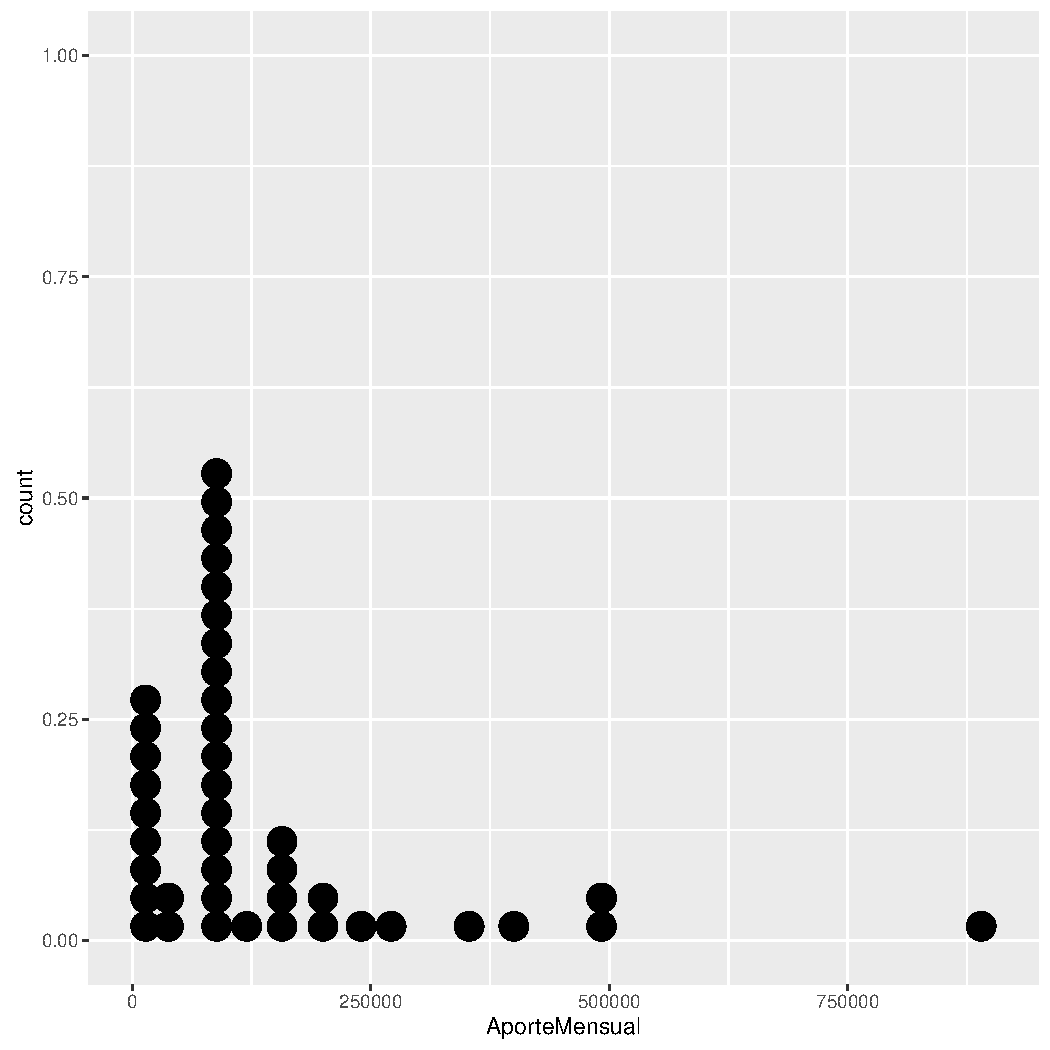
\includegraphics[width=\maxwidth]{figure/MontosAportes-1} 

\end{knitrout}
	\caption{Comportamiento de la variable Monto Aportado al Sistema de Seguridad Social}
\end{figure}

De acuerdo con los datos de la gr\'{a}fica, se observan aportes entre el rango de 98 a 890.000 pesos colombianos.  Los montos de los aportes empiezan con valores menores a la media, es decir 84.000 pesos, posteriormente, se observa el mayor incremento de los aportes en 140.000 pesos y luego comienzan a disminuir hasta los 250.000 pesos colombianos.  Seguidamente, se observan valores alrededor de lo 350.000 y 500.000 pesos colombianos y finalmente, se observa un registro de 890.000 pesos colombianos.  
De acuerdo con los datos observados, los colombianos tiene un aporte bajo al sistema de Seguridad Social y se concentra alrededor de la media es decir 140.000 pesos colombianos.


Con fundamento en los resultados preliminares previos, realizaremos un an\'{a}lisis del conjunto de datos m\'{a}s al detalle, de acuerdo con la informaci\'{o}n disponible.

\vspace{-0mm}
\subsection{Analizando población que aporta al Sistema de Seguridad Social Colombiano cuya edad comprende el rando de 72 hasta 94 años.}

Al comparar la media del total de la poblaci\'{o}n de ciudadanos que aportan al sistema de seguridad social colombiano con la media de la poblaci\'{o}n cuya edad est\'{a} entre 72 a 94 años se observa un incremento de 116.794 pesos colombianos al pasar de 140.206 pesos colombianos a 257.584 pesos colombianos, respectivamente, con lo cual, preliminarmente confirmamos que aumenta el monto de los valores cotizados a este sistema conforme la edad del aportante aumenta. 


%Los datos más representativos se dan a continuación:

% Table created by stargazer v.5.2 by Marek Hlavac, Harvard University. E-mail: hlavac at fas.harvard.edu
% Date and time: vie, jun 03, 2016 - 05:04:04 p.m.
\begin{table}[!htbp] \centering 
  \caption{Total de la población de aportantes al sistema de seguridad social con edad entre 72 y 94 años.} 
  \label{} 
\begin{tabular}{@{\extracolsep{5pt}}lccccc} 
\\[-1.8ex]\hline 
\hline \\[-1.8ex] 
Statistic & \multicolumn{1}{c}{N} & \multicolumn{1}{c}{Mean} & \multicolumn{1}{c}{St. Dev.} & \multicolumn{1}{c}{Min} & \multicolumn{1}{c}{Max} \\ 
\hline \\[-1.8ex] 
TotalAportes & 5 & 257,584.200 & 364,146.600 & 99 & 890,000 \\ 
Genero & 5 & 1.200 & 0.447 & 1 & 2 \\ 
Edad & 5 & 76.200 & 3.421 & 72 & 81 \\ 
\hline \\[-1.8ex] 
\end{tabular} 
\end{table} 


\vspace{1mm}
{\footnotesize \textbf{Convenciones:} Genero) 1: Mujer, 2: Hombre; Edad) Edad del Aportante Analizado.}

De acuerdo con la gr\'{a}fica, se observa un aportante con edad superior a 80 años quien aporta al sistema de seguridad social colombiano. Al comparar el conjunto de datos de los aportes al sistema de seguridad social colombiano con este monto aportado, se observa que este dato tiene una caracter\'{i}stica \'{u}nica por ser quien aport\'{o} el mayor monto al sistema de seguridad social de acuerdo con la informaci\'{o}n analizada. 

%\vspace{0mm}
\begin{figure}[H]
	\centering
\begin{knitrout}
\definecolor{shadecolor}{rgb}{0.969, 0.969, 0.969}\color{fgcolor}
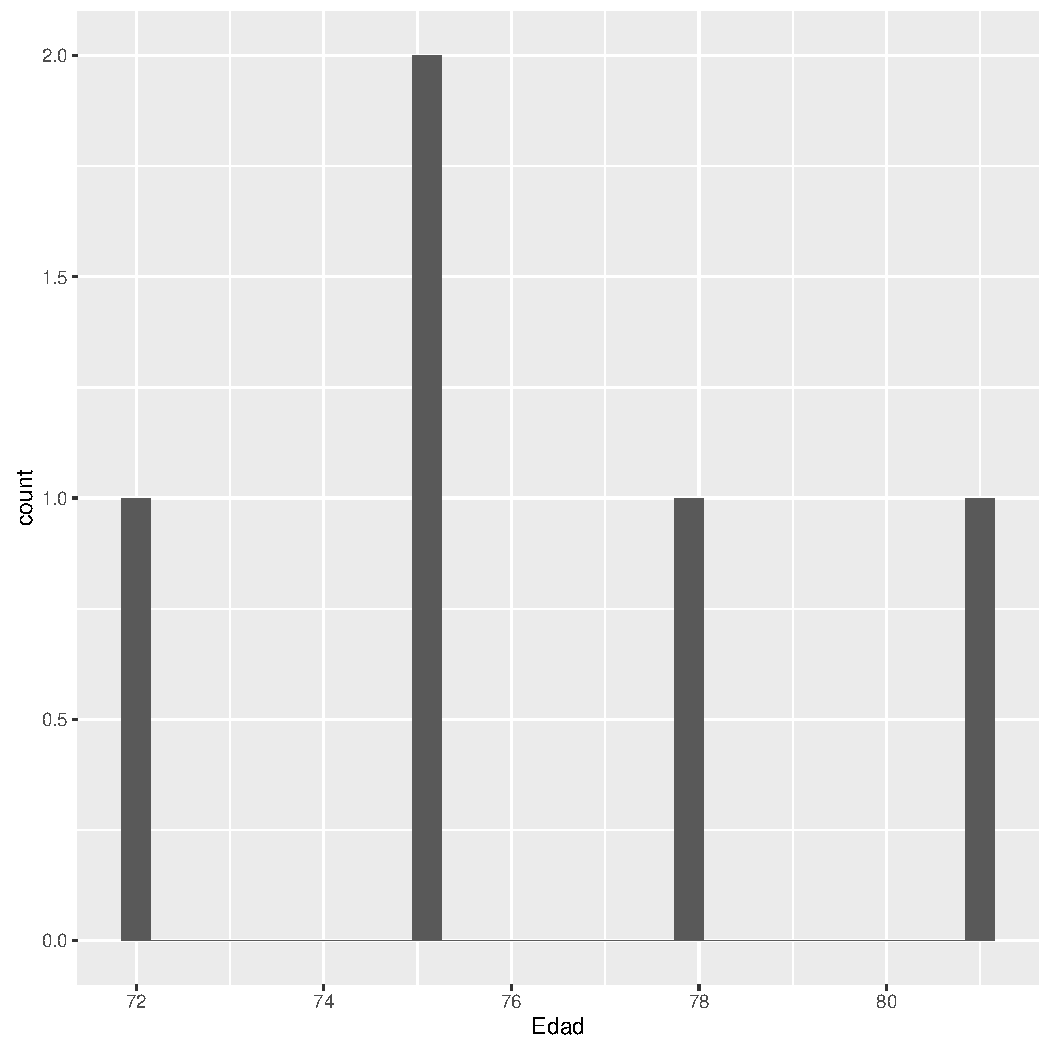
\includegraphics[width=\maxwidth]{figure/Aportantes1943-1} 

\end{knitrout}
	\caption{Población de aportantes del sistema de seguridad social con edad entre 72 y 94 años.}
\end{figure}

Adicionalmente, en la siguiente gr\'{a}fica se observa, que los aportes de los ciudadamos cuya edad est\'{a} entre 72 y 94 años presentan una brecha entre el valor m\'{a}ximo y la media para este rango, existiendo una diferencia de 633.000 pesos colombianos al pasar de 257.000 a 890.000 pesos colombianos, respectivamente.  Tambi\'{e}n, se observa  en la distribuci\'{o}n de los montos aportados, la mayor diferencia entre el menor y el mayor valor aportado, evidenciando la diferencia social de los aportes para esta categor\'{i}a de datos analizados.

Al comparar los datos de la gr\'{a}fica de la variable edad y la variable valor aportado, se observa que la primera tiene una distribuci\'{o}n uniforme, mientras que la segunda evidencia una inclinaci\'{o}n de los datos a la izquierda, concentrado los datos antes de los 250.000 pesos colombianos, y evidenciando que el valor m\'{a}ximo se presenta con poca frecuencia como aporte al sistema social colombiano.   


%\vspace{0mm}
\begin{figure}[H]
	\centering
\begin{knitrout}
\definecolor{shadecolor}{rgb}{0.969, 0.969, 0.969}\color{fgcolor}
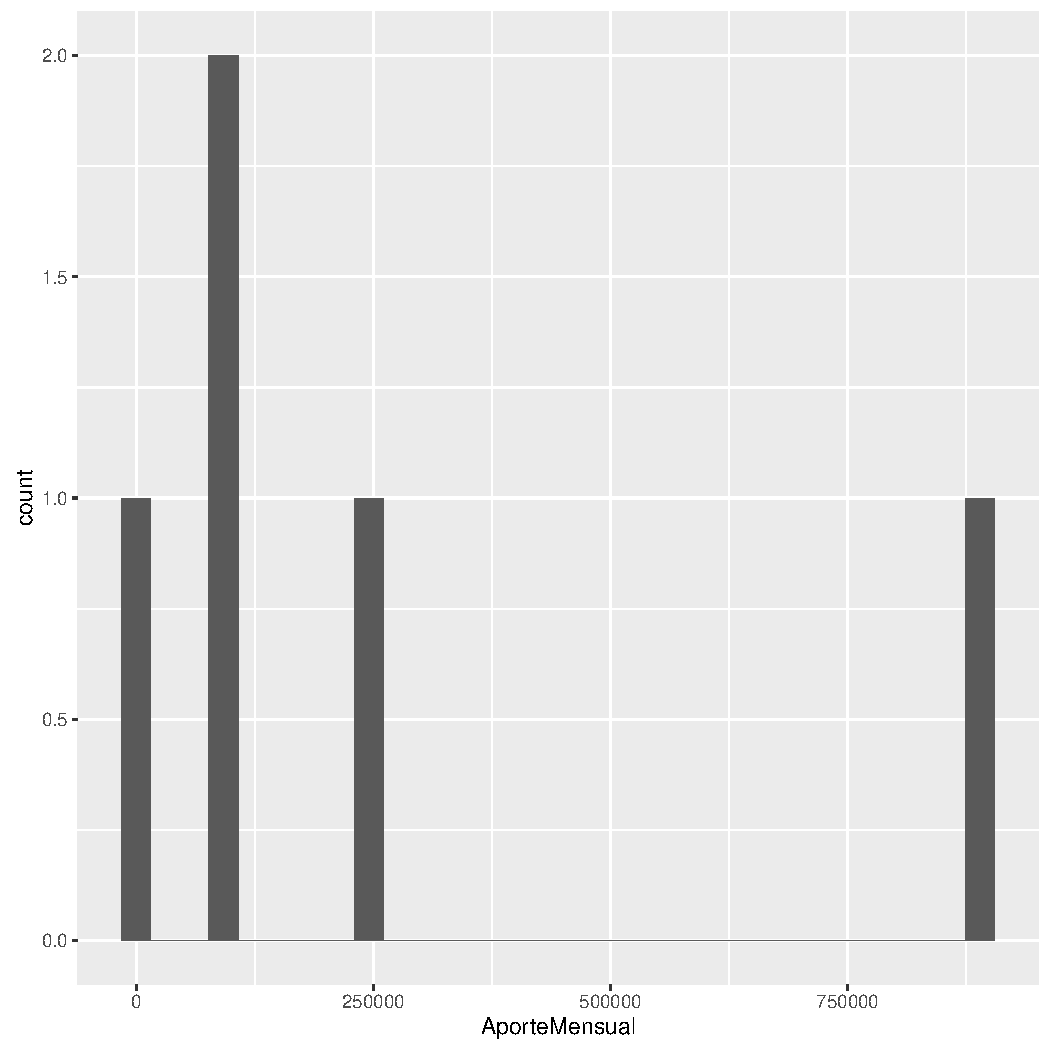
\includegraphics[width=\maxwidth]{figure/MontoAporte1943-1} 

\end{knitrout}
	\caption{Montos de los aportes al sistema de seguridad social de la poblacion con edad entre 72 y 94 años.}
\end{figure}




%\vspace{-10mm}
\subsection{Analizando población  que aporta al Sistema de Seguridad Social Colombiano cuya edad comprende el rango de 50 años y menos de 71 años.}

%Los datos más representativos se dan a continuación:

% Table created by stargazer v.5.2 by Marek Hlavac, Harvard University. E-mail: hlavac at fas.harvard.edu
% Date and time: vie, jun 03, 2016 - 05:04:04 p.m.
\begin{table}[!htbp] \centering 
  \caption{Total de la poblacion de aportantes del sistema de seguridad social con edad entre 50 y 71 años.} 
  \label{} 
\begin{tabular}{@{\extracolsep{5pt}}lccccc} 
\\[-1.8ex]\hline 
\hline \\[-1.8ex] 
Statistic & \multicolumn{1}{c}{N} & \multicolumn{1}{c}{Mean} & \multicolumn{1}{c}{St. Dev.} & \multicolumn{1}{c}{Min} & \multicolumn{1}{c}{Max} \\ 
\hline \\[-1.8ex] 
TotalAportes & 16 & 169,552.000 & 160,928.200 & 98 & 492,000 \\ 
Genero & 16 & 1.562 & 0.512 & 1 & 2 \\ 
Edad & 16 & 59.438 & 5.329 & 50 & 66 \\ 
\hline \\[-1.8ex] 
\end{tabular} 
\end{table} 


\vspace{1mm}
{\footnotesize \textbf{Convenciones:} Genero) 1: Mujer, 2: Hombre; Edad) Edad del Aportante Analizado.}

Al comparar la media del total de la poblaci\'{o}n de ciudadanos que aportan al Sistema de Seguridad Social Colombiano con la media de la poblaci\'{o}n cuya edad est\'{a} entre 50 y 71 años, se observa un incremento de 29.346 pesos colombianos al pasar de 140.206 pesos colombianos a 169.552 pesos colombianos, respectivamente, con lo cual, continua la tendencia, al aumentar el monto de los valores cotizados a este sistema conforme la edad del aportante aumenta. 


Basados en los datos de la siguiente gr\'{a}fica, se observa constancia en el n\'{u}mero de aportantes que existen para el rango de los ciudadanos con edad entre 50 a 59 años, y un incremento en el n\'{u}mero de aportantes en el rango de 60 a 71 años.  Llama la atenci\'{o}n el incremento del n\'{u}mero de aportantes a los 71 años, lo cual corresponden a ciudadanos pensionados por el Sistema de Seguridad Social Colombiano.  

%\vspace{-5mm}
\begin{figure}[H]
	\centering
\begin{knitrout}
\definecolor{shadecolor}{rgb}{0.969, 0.969, 0.969}\color{fgcolor}
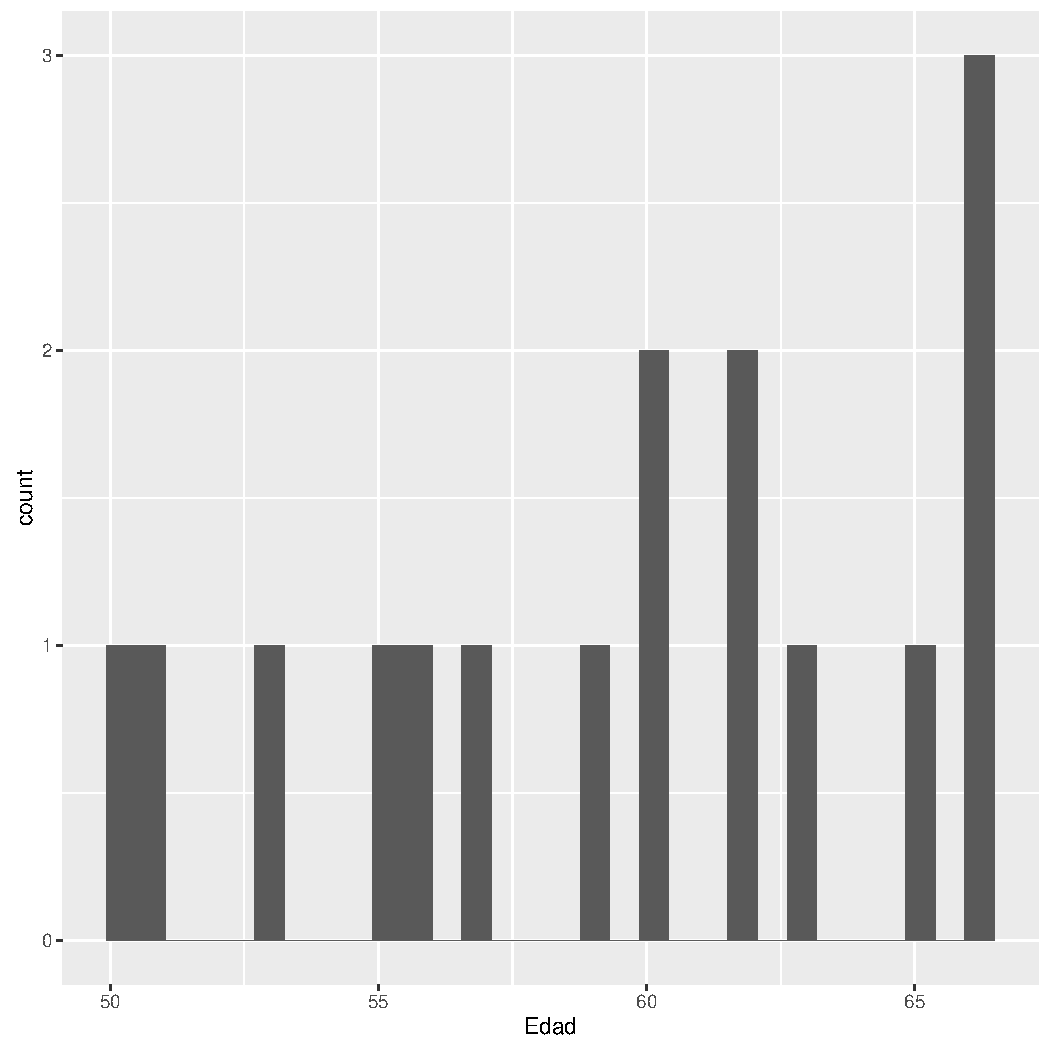
\includegraphics[width=\maxwidth]{figure/Aportantes1965-1} 

\end{knitrout}
	\caption{Población de aportantes del sistema de seguridad social con edad entre 50 y 71 años.}
\end{figure}

Tambi\'{e}n revisaremos la calidad de los aportes realizado al sistema de acuerdo con los datos de este rango, presentados en la siguiente gr\'{a}fica:


%\vspace{-5mm}
\begin{figure}[H]
	\centering
\begin{knitrout}
\definecolor{shadecolor}{rgb}{0.969, 0.969, 0.969}\color{fgcolor}
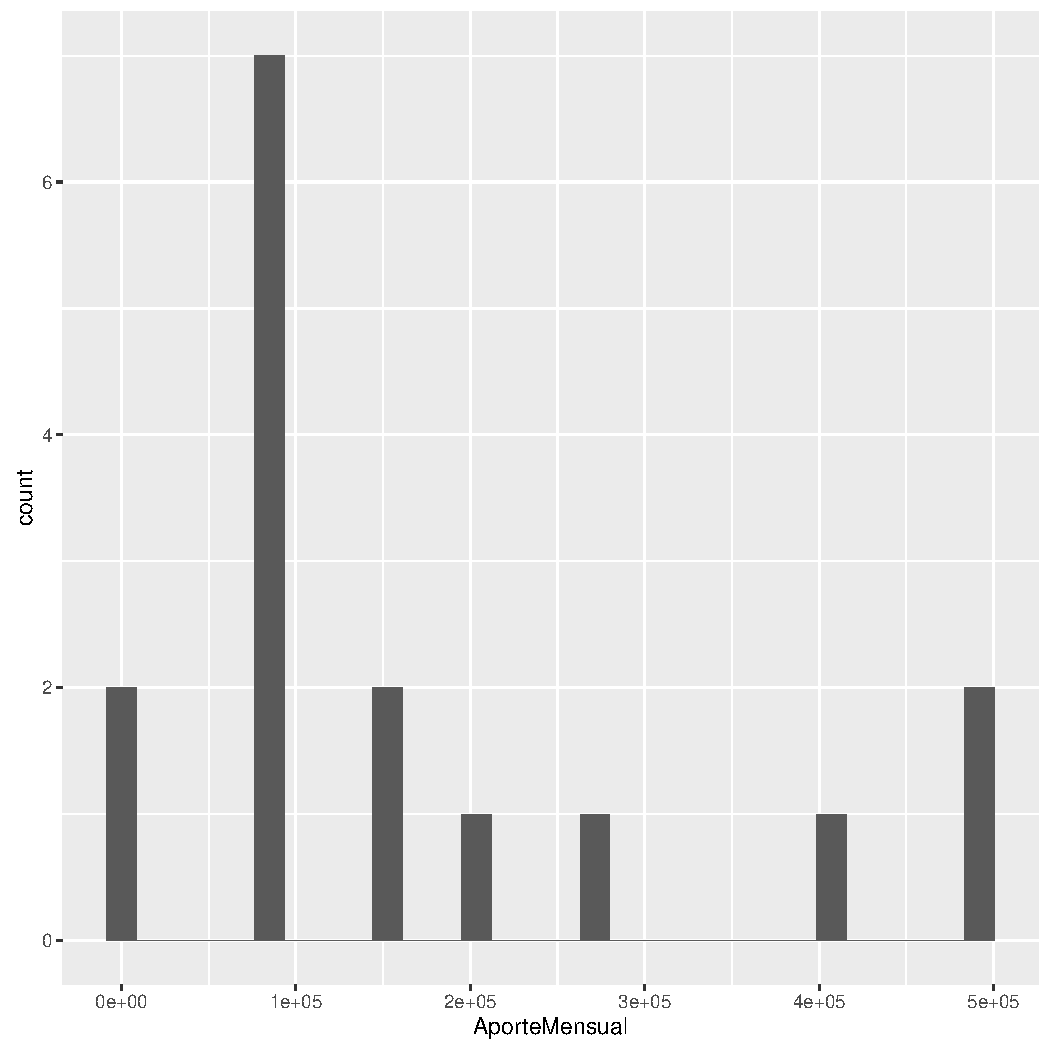
\includegraphics[width=\maxwidth]{figure/Aportantes1965monto-1} 

\end{knitrout}
	\caption{Montos de los aportes al sistema de seguridad social con edad entre 50 y 71 años.}
\end{figure}

Al comparar la media del total de la poblaci\'{o}n de ciudadanos que aportan al Sistema de Seguridad Social Colombiano con la media de la poblaci\'{o}n cuya edad est\'{a} entre 50 a 71 años, se observa un incremento de 29.346 pesos colombianos al pasar de 140.206 pesos colombianos a 169.552 pesos colombianos, respectivamente. 

%\vspace{-10mm}
\subsection{Analizando población de aportantes del sistema de seguridad social con edad entre 27 y 50 años.}
%Los datos más representativos se dan a continuación:

% Table created by stargazer v.5.2 by Marek Hlavac, Harvard University. E-mail: hlavac at fas.harvard.edu
% Date and time: vie, jun 03, 2016 - 05:04:05 p.m.
\begin{table}[!htbp] \centering 
  \caption{Total de la población de aportantes al sistema de seguridad social con edad entre 27 y 50 años.} 
  \label{} 
\begin{tabular}{@{\extracolsep{5pt}}lccccc} 
\\[-1.8ex]\hline 
\hline \\[-1.8ex] 
Statistic & \multicolumn{1}{c}{N} & \multicolumn{1}{c}{Mean} & \multicolumn{1}{c}{St. Dev.} & \multicolumn{1}{c}{Min} & \multicolumn{1}{c}{Max} \\ 
\hline \\[-1.8ex] 
TotalAportes & 17 & 100,798.200 & 85,902.920 & 98 & 353,200 \\ 
Genero & 17 & 1.412 & 0.507 & 1 & 2 \\ 
Edad & 17 & 38.235 & 6.978 & 27 & 49 \\ 
\hline \\[-1.8ex] 
\end{tabular} 
\end{table} 


\vspace{1mm}
{\footnotesize \textbf{Convenciones:} Genero) 1: Mujer, 2: Hombre; Edad) Edad del Aportante Analizado.}

Al comparar la media de los aportes del total de la poblaci\'{o}n de ciudadanos que aportan al Sistema de Seguridad Social Colombiano con la media de la poblaci\'{o}n cuya edad est\'{a} entre 27 a 50 años, se observa un disminuci\'{o}n de 39.408 pesos colombianos al pasar de 140.206 pesos colombianos a 100.798 pesos colombianos, respectivamente, con lo cual, continua la tendencia, al aumentar el monto de los valores cotizados a este sistema conforme la edad del aportante aumenta. 


%\vspace{-5mm}
\begin{figure}[H]
	\centering
\begin{knitrout}
\definecolor{shadecolor}{rgb}{0.969, 0.969, 0.969}\color{fgcolor}
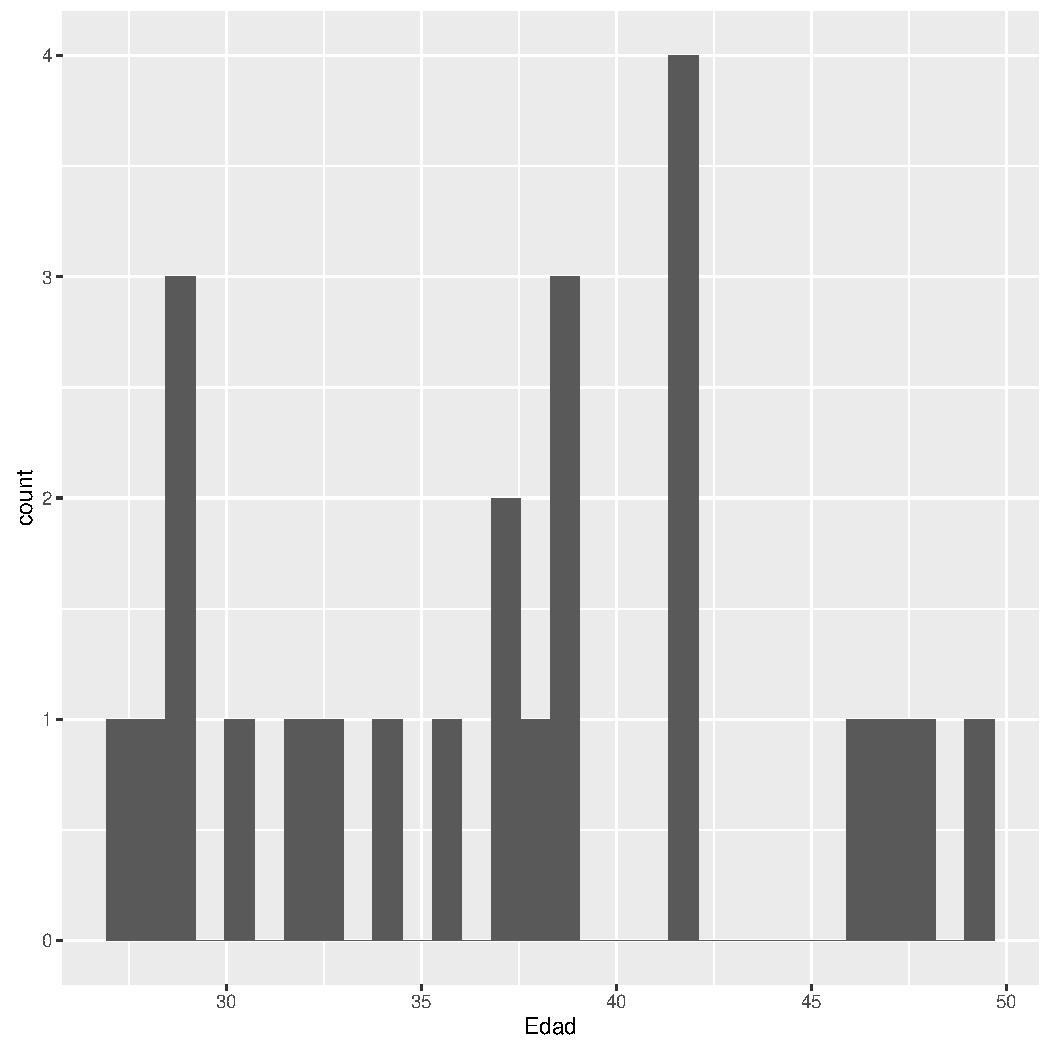
\includegraphics[width=\maxwidth]{figure/Aportantes1988-1} 

\end{knitrout}
	\caption{Población de aportantes del sistema de seguridad social con edad entre 27 y 50 años.}
\end{figure}

Al revisar los montos aportados en este rango, se observa una gr\'{a}fica inclinada a la izquierda, indicando que el valor de los montos est\'{a}n sobre los 100.000 pesos colombianos. Tambi\'{e}n, se observa un \'{u}nico dato de 353,200 para este rango de datos evidenciando una diferencia social entre el m\'{a}ximo valor y la media de los aportes al sistema de seguridad social colombiano en este rango de datos analizado.


%\vspace{-5mm}
\begin{figure}[H]
	\centering
\begin{knitrout}
\definecolor{shadecolor}{rgb}{0.969, 0.969, 0.969}\color{fgcolor}
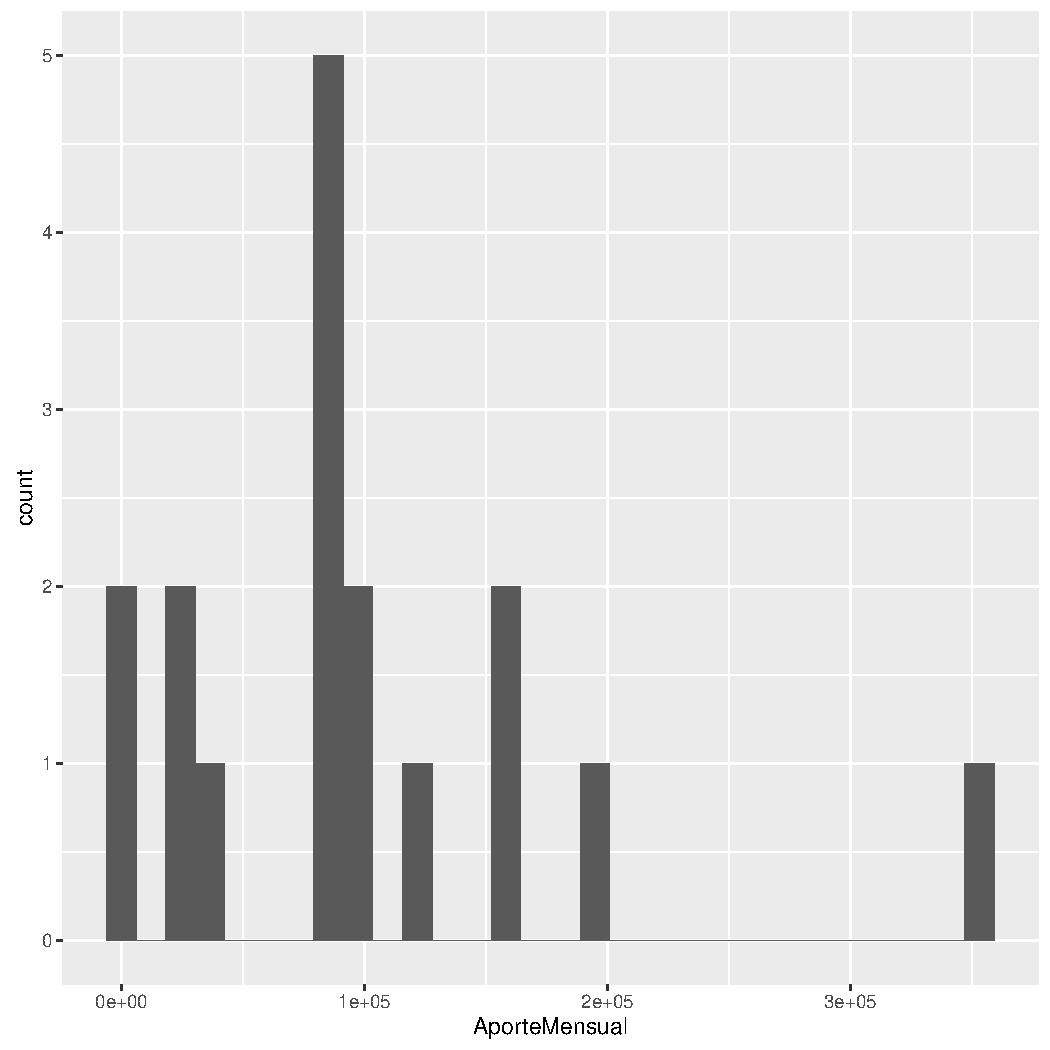
\includegraphics[width=\maxwidth]{figure/Aportantes1988monto-1} 

\end{knitrout}
	\caption{Montos de los aportes al sistema de seguridad social con edad entre 27 y 50 años.}
\end{figure}


%\vspace{-10mm}
\subsection{Analizando población de aportantes del sistema de seguridad social con edad entre 22 y 26 años.}
%Los datos más representativos se dan a continuación:

% Table created by stargazer v.5.2 by Marek Hlavac, Harvard University. E-mail: hlavac at fas.harvard.edu
% Date and time: vie, jun 03, 2016 - 05:04:06 p.m.
\begin{table}[!htbp] \centering 
  \caption{Total de la población de aportantes del sistema de seguridad social con edad entre 22 26 años.} 
  \label{} 
\begin{tabular}{@{\extracolsep{5pt}}lccccc} 
\\[-1.8ex]\hline 
\hline \\[-1.8ex] 
Statistic & \multicolumn{1}{c}{N} & \multicolumn{1}{c}{Mean} & \multicolumn{1}{c}{St. Dev.} & \multicolumn{1}{c}{Min} & \multicolumn{1}{c}{Max} \\ 
\hline \\[-1.8ex] 
TotalAportes & 4 & 43,587.000 & 26,988.470 & 25,774 & 82,800 \\ 
Genero & 8 & 1.375 & 0.518 & 1 & 2 \\ 
Edad & 8 & 23.250 & 1.389 & 22 & 26 \\ 
\hline \\[-1.8ex] 
\end{tabular} 
\end{table} 

\vspace{1mm}
{\footnotesize \textbf{Convenciones:} Genero) 1: Mujer, 2: Hombre; Edad) Edad del Aportante Analizado.}

Basados en los resultados de la tabla anterior, observamos que al comparar la media de los montos aportados al Sistema de Seguridad Social por el total de la poblaci\'{o}n de ciudadanos  con relaci\'{o}n a la media de la poblaci\'{o}n cuya edad est\'{a} entre 22 a 26 años, identificamos una disminuci\'{o}n de 96.616 pesos colombianos al pasar de 140.206 pesos colombianos a 43.587 pesos colombianos, respectivamente, con lo cual, continua la tendencia donde aumenta el monto de los valores cotizados considerando la variable edad del aportante.

Al analizar como es la distribucin\'{o}n de los datos en este rango, analizando la variable edad observamos que existen un mayor n\'{u}mero de  aportantes hacia los 22 años y que el n\'{u}mero de incidencias disminuye hacia los 26 años, como se observa en la siguiente gr\'{a}fica: 

%\vspace{-10mm}
\begin{figure}[H]
	\centering
\begin{knitrout}
\definecolor{shadecolor}{rgb}{0.969, 0.969, 0.969}\color{fgcolor}
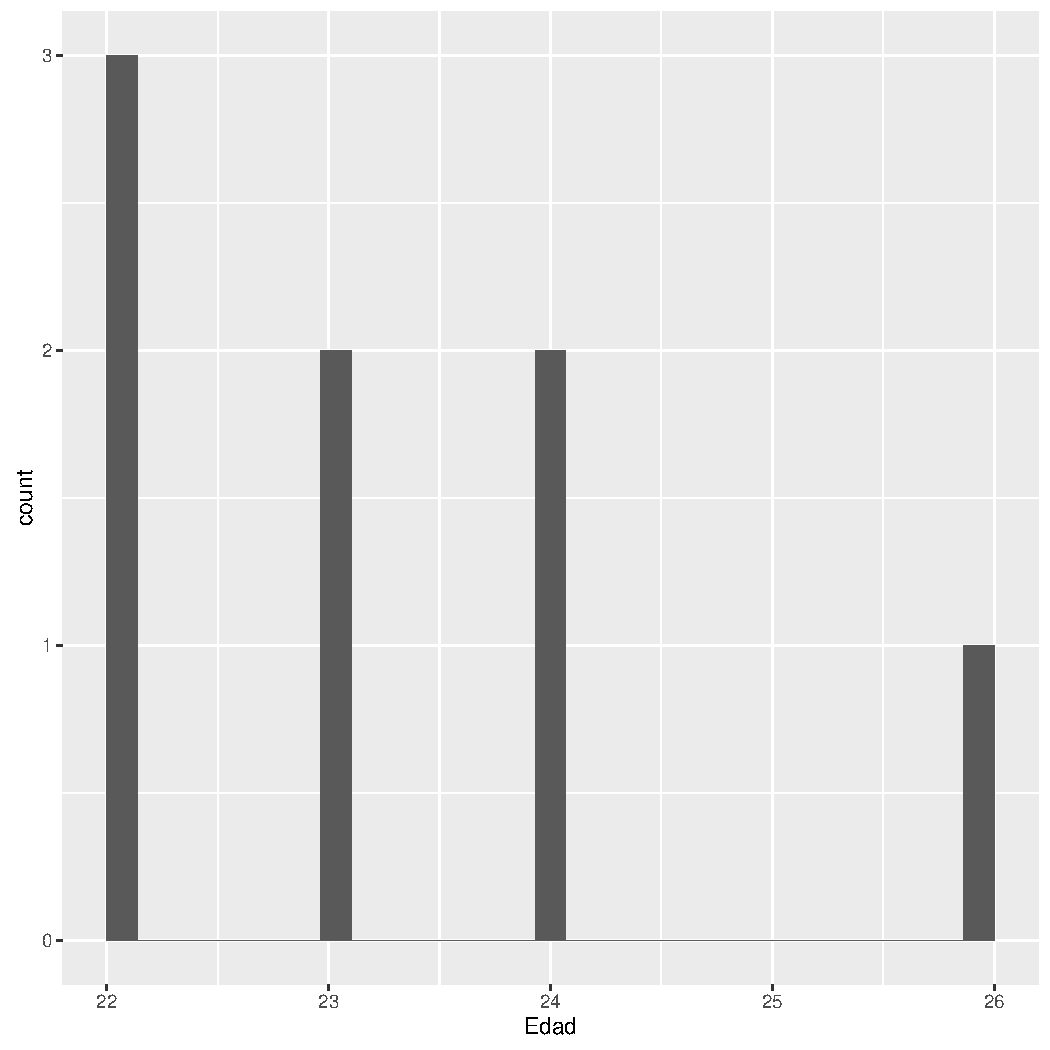
\includegraphics[width=\maxwidth]{figure/Aportantes1993-1} 

\end{knitrout}
	\caption{Población de aportantes del sistema de seguridad social con edad entre 22 y 26 años.}
\end{figure}

Tambi\'{e}n, analizamos el comportamiento de los montos aportados, al sistema observando una inclinaci\'{o}n de los datos hacia  la izquierda, observando una mayor incidencia alrededor de los  25.774 pesos colombianos, como se observa a continuaci\'{o}n.

%\vspace{-10mm}
\begin{figure}[H]
	\centering
\begin{knitrout}
\definecolor{shadecolor}{rgb}{0.969, 0.969, 0.969}\color{fgcolor}
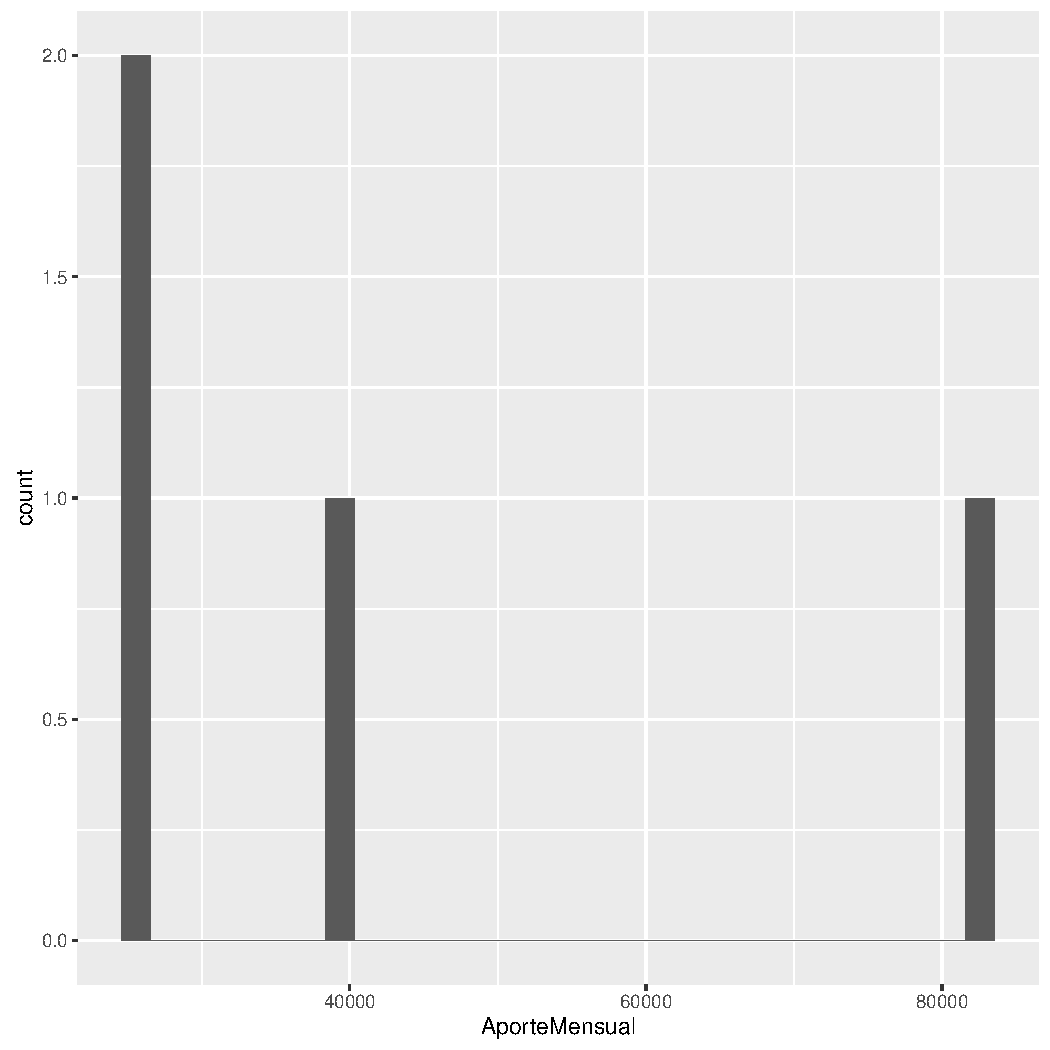
\includegraphics[width=\maxwidth]{figure/Aportantes1993monto-1} 

\end{knitrout}
	\caption{Montos de los aportes del sistema de seguridad social con edad entre 22 y 26 años.}
\end{figure}

Finalmente se presenta los montos aportados al sistema de seguridad social colombiano categorizado por la varible Edad. 

\begin{itemize}
	\item Promedio de montos de los aportes de los ciudadanos entre 22 a 26 años:
[1] 43587

	\item Promedio de montos de los aportes de los ciudadanos entre 27 a 50 años:
[1] 100798.2

	\item Promedio de montos de los aportes de los ciudadanos entre 51 a 71 años:
[1] 169552

	
	\item Promedio de montos de los aportes de los ciudadanos entre 72 a 94 años:
[1] 257584.2

	
	\item Promedio de montos de los aportes de los ciudadanos al Sistema de Seguridad Social presentado de forma consolidada:
[1] 140206.5

\end{itemize}

\section{An\'{a}lisis Exploratorio}

Revisado los resultados del trabajo realizado observamos que el valor m\'{a}ximo de los aportes realizados por la poblaci\'{o}n colombiana al sistema de seguridad social aumentan con relaci\'{o}n a la variable Edad, al pasar: 

\begin{itemize}
	
	\item  de 82.800 pesos colombianos para el rango de aportantes de 22 a 26  años
	
	
	\item  de 353.200 pesos colombianos para el rango de aportantes de 27 a 50  años
	
	\item  de 492.000 pesos colombianos para el rango de aportantes de 51 a 71  años
	
	\item  de 890.000 pesos colombianos para el rango de aportantes de 72 a 94  años.
	
\end{itemize}

En consecuencia, se puede concluir que existe un n\'{u}mero de ciudadanos a los cuales sus aportes est\'{a}n por encima de la media de los montos de los aportes al sistema y aumentan con relaci\'{o}n a la variable edad. 

\section{An\'{a}lisis Inferencial}

Finalmente, fundamentados en los resultados obtenidos en fases previas, consideramos la pregunta donde se cuestiona s\'{i} los colombianos que m\'{a}s aportan tienen una edad mayor a 30 años, a la cual podemos mencionar:  


\begin{itemize}
	
	\item  La media de los montos aportados al sistema de seguridad social colombiano con datos al 2015, categorizados por rangos, aumentan con relaci\'{o}n a la variable edad.
	
	\item  Los valores m\'{a}ximos de los montos aportados aumentan con relaci\'{o}n a la variable edad.
	
	\item   Al revisar, la gr\'{a}fica que consolida los montos de los aportes de los ciudadanos entre 22 y 26  años se observa una media de 43.587 pesos colombianos y un valor m\'{a}ximo de 82.800 pesos colombianos, respectivamente, con lo cual estos valores son menores a los aportes en otras categor\'{i}as analizados en este papel. 
	
\end{itemize}  

En consecuencia se concluye que los montos aportados al sistema de seguridad social colombiano, por los ciudadanos con edad superior a 30 años es mayor a los montos aportados por la poblaci\'{o}n con una edad menor.

Finalmente, mediante el an\'{a}lisis de la informaci\'{o}n mediante la t\'{e}cnica de miner\'{i}a de datos K-means, el cual permite visualizar el comportamiento de las variables Edad y Monto aportado en Conjunto, as\'{i}: 

\begin{kframe}


{\ttfamily\noindent\bfseries\color{errorcolor}{\#\# Error in eval(expr, envir, enclos): no se pudo encontrar la funci�n "{}geom.dotplot"{}}}\end{kframe}
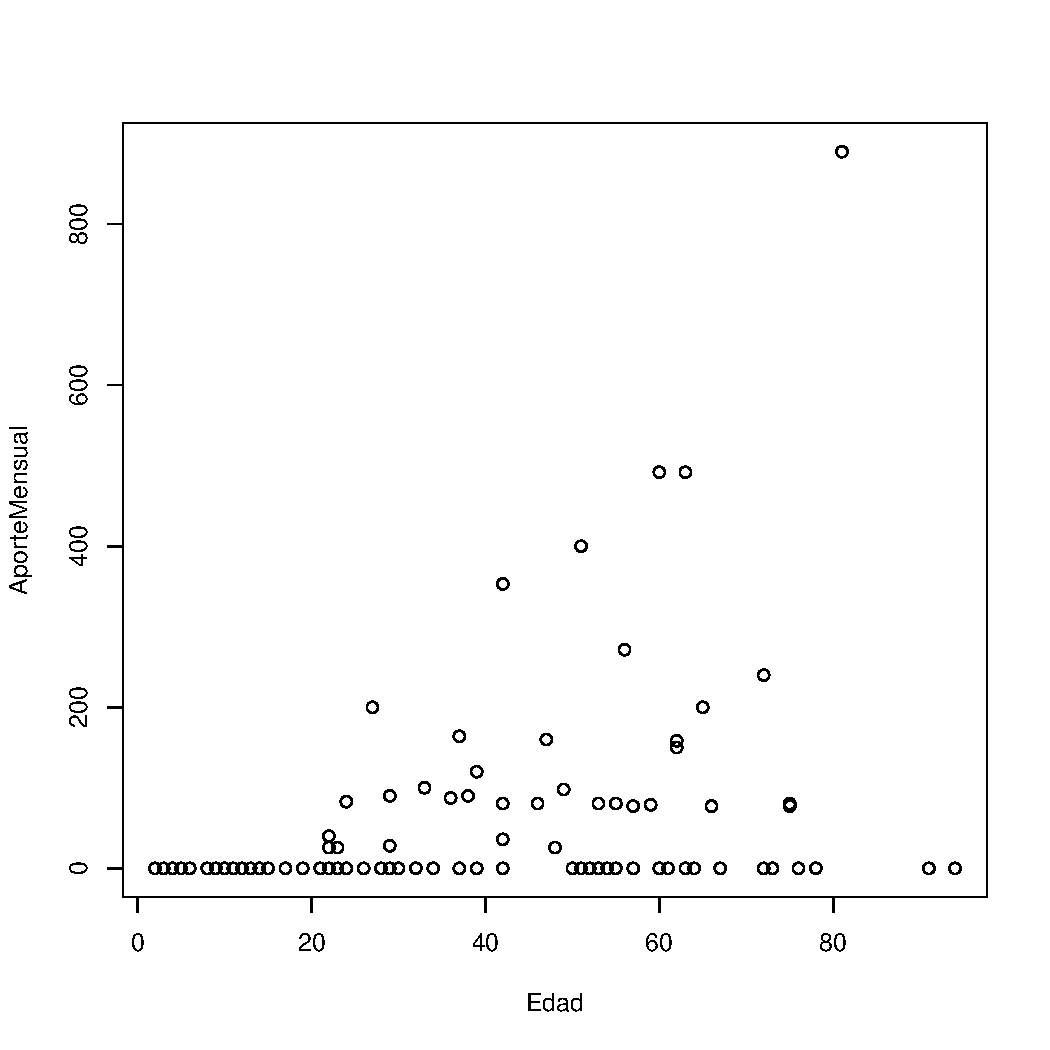
\includegraphics[width=\maxwidth]{figure/medias-1} 



En el eje de las X, se observa la variable edad y en en el eje de la y, se representa la variable de los aportes al sistema, la cual sintetiza el an\'{a}lisis realizado.



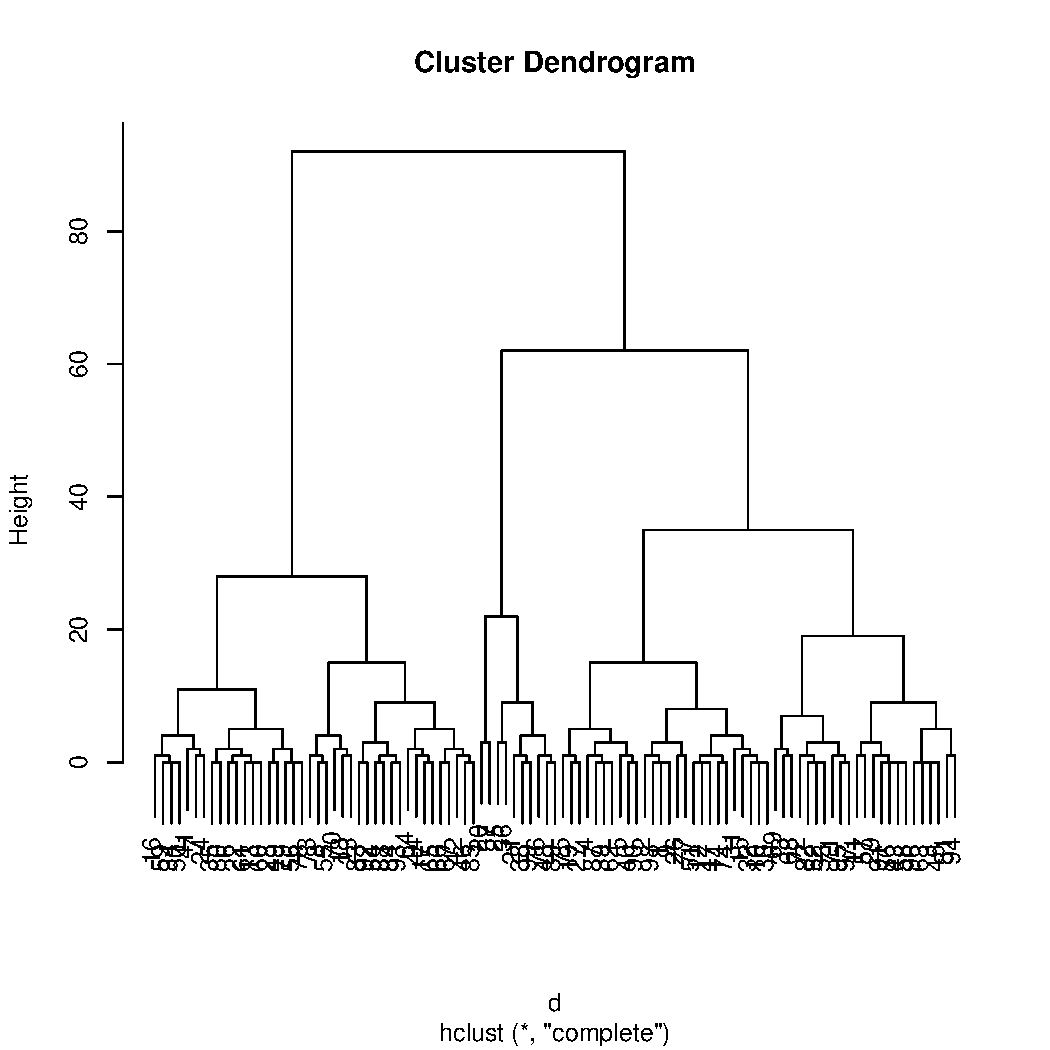
\includegraphics[width=\maxwidth]{figure/dendogran-1} 




	



%Resultados
%SECCIÓN 4. Resultados
\section{Conclusiones}

En este papel se confirmó que el monto del valor aportado al Sistema de Seguridad Social Colombiano aumentaba con relación a la variable edad. De acuerdo con los resultados, después de los 50 años, los monos de los aportes superan los 140.000 pesos colombiano, cifra que corresponde a la media de los aportes sistema de seguridad social. También de induce de los resultados que los ciudadanos mayores que son pensionados o próximos a lograr su pensión realizan aportes por encima de la media es decir 140.000 pesos colombianos.  Con los resultados obtenidos se confirma la pregunta de investigación asociada con el monto de los aportes de los afiliados al sistema de seguridad social y su relación con la variable edad del cotizante. 

Con este análisis, también se confirma que los datos abiertos publicados por entes gubernamentales contribuyen a generar servicios con valor social, en razón a que el uso de este tipo de información permite la toma de decisiones soportados en datos que cumplen con las características de los datos abiertos. 

De otro lado, con los resultados de este papel, se concluye que los datos expuestos por el DANE, el análisis realizado y las técnicas de minería de datos permitieron confirmar la calidad de la información generada por esta entidad gubernamental del estado Colombiano. 

Finalmente, es importante resaltar que se logró brindar un resultados producto de un proceso de análisis basados en el marco metodológico expuesto por área de conocimiento con es la minería de datos, la cual brindó las herramientas para el procesos de validación de la calidad de los datos y la verificación y confirmación de la pregunta de investigación


\section{Trabajos futuros} 


Este trabajo permite definir trabajos adicionales que brinde certeza de la sostenibilidad del sistema y como el estado colombiano debe tomar acción para garantizar la sostenibilidad de este modelo de seguridad social Colombiano. 

	%BIBLIOGRAFÍA
	%ENTORNO {thebibliography}
	%Permite al autor listar las referencias utilizadas y citarlas en algun punto del texto.

	

	 \begin{thebibliography}{1}
	 	
		\bibitem{biblio1}
		Davies, Tim. (2011). What’s in the Linked Open Data Stack? Open Data Impacts. The research blog of Tim Davies. (Pág. 270) 	
	 	
		\bibitem{biblio2}
		MinTIC. Ministerio de Tecnologías de la Información y las Comunicaciones de la República de Colombia. (2011). Entregable No. 2: Lineamientos para la implementación de datos abiertos en Colombia.  
		
		\bibitem{biblio3}
		Opengovdata. Open Government Data. (2007). The Annotated 8 Principles of Open Government Data.
	 	
	 	\bibitem{biblio4}
	 	Rodriguez,  L. A., Cueva, J. M., Tarazona, G. M., & Montenegro, C. E. (2013a). Open Data as a key factor for developing expert systems: a perspective from Spain. International Journal of Interactive Multimedia and Artificial Intelligence, 2(2), (Pág. 51-55.)
	 	
	 	\bibitem{biblio5}
	 	Rodriguez, L. A., Tarazona, G. M., & Cueva, J. M. (2014). Open Data and Big Data: A Perspective from Colombia. En L. Uden et al. (Eds.),  Knowledge Management in Organizations. 9th International Conference, KMO 2014, Santiago, Chile, September 2-5, 2014, Proceedings, (Pág. 35-41).
	 	
	 	\bibitem{biblio6}
	 	W3C. World Wide Web Consortium. (2009). Publishing Open Government Data. 
	 	
		\bibitem{biblio7}
	 	S. Sumathi., S. Esakkirajan., (2007). Data Mining and Data Warehousing. (Pág. 1-30)
	 	
	 	\bibitem{biblio8}
	 	M. ferri, J. Hernández.; C. Ramírez, Introducción a la Minería de Datos. Prentice Hall. España, 2004
	 	
	 	\bibitem{biblio9}
	 	Public.Resource.Org. (2007). Open Government Data Principles. URL:  
	 	
	 \end{thebibliography}
	
\end{document}
